\documentclass[../thesis.tex]{subfiles}
% !TeX spellcheck = fr_FR

\begin{document}
	\chapter{Indices de végétation}
	\label{chap:vegetation-indices}
	
	Dans le chapitre précédent, nous avons vu comment pré-traiter les données en vue de leur exploitation. La seconde étape de notre chaîne de traitement vise à répondre à la question suivante : comment discriminer la végétation du reste de la scène ? Pour répondre à cette question, l'approche classique repose sur l'utilisation d'indices de végétation, sur lesquels une méthode de segmentation simple est appliquée, telle qu'un seuillage. Comme nous l'avons vu dans le chapitre \ref{chap:computer-vision}, la définition de tels indices (parmi lesquels le NDVI est le plus connu) repose essentiellement sur des connaissances empiriques \cite{bannari1995review} (section \ref{sec:vegetation-indices}). Ces indices utilisent souvent des données calibrées en réflectance, censées garantir leur stabilité.

    Or de nombreux facteurs influencent de tels indices de télédétection. La calibration radiométrique et le capteur sont deux facteurs importants dans l'estimation de ces indices. \cite{lee2021comparison} montre leurs effets au cours de la journée sur le NDVI. Cet indice peut varier d'un facteur de $\SI{20}{\percent}$ après correction de ces deux paramètres. D'autres facteurs, comme les conditions atmosphériques, l'humidité de la végétation, l'humidité du sol, la couverture végétale globale, l'ombre et les différences de type de sol, jouent aussi des rôles importants dans l'estimation du couvert végétal. Par exemple, la lumière réfléchie par le sol et l'ombre obscurcissant partiellement une image, peuvent influencer les valeurs du NDVI dans une large mesure \cite{Zhang2015}, rendant difficile l'utilisation d'un tel indice.
    
    Ces limitations ont été la raison du développement de nombreux indices de végétation, ajustés au sol (par exemple, Soil-Adjusted Vegetation Index, Modified Soil-Adjusted Vegetation Index) ou à l'atmosphère (Atmospherically Resistant Vegetation Index) \cite{bannari1995review}. Ces modèles, plus robustes, restent néanmoins fortement limités et influencés par tous ces facteurs. L'utilisation d'un seuillage fixe est donc peu pertinente car il faut s'attendre à des valeurs différentes pour une même zone d'observation au fil du temps, en raison des changements environnementaux affectant l'observation (saisonniers, phénologiques, météorologique, \dots).
    
    %Dit autrement, les indices de télédétection sont une transformation des images d'entrée, qui prend une quantité limitée d'informations de l'entrée. Ainsi, les indices spectraux entraînent une perte d'informations discriminantes essentielles à la classification, lors de la transformation. Les indices spectraux sont fortement limités par ce simple fait.
    
    Pour augmenter la performance de cette étape de traitement, certains utilisent une méthode de classification faisant appel à plusieurs indices usuels \cite{Shishir2018, Gee2021}. D'autres en revanche, utilisent des algorithmes génétiques afin d'apprendre l'équation idéale permettant une segmentation optimale \cite{GeneticKabiri, GeneticAlbarracin}. Dans les deux cas, cela revient à prendre en considération une plus large quantité d'information, ce qui augmente le potentiel de discrimination. En revanche, l'optimisation de ces indices utilise des méthodes, soit coûteuses en temps, soit ne garantissant pas un optimum, les rendant peu applicables à de larges bases de données.
    
    Face à ce constat, une nouvelle méthodologie est proposée dans ce chapitre pour l'apprentissage de tels indices. Elle repose sur l'apprentissage d'approximateurs de fonctions. Ainsi, on cherche une fonction qui peut décrire toutes les autres. Cette approche peut être mise en œuvre en apprentissage profond. Ce qui permet d'exploiter le processeur graphique, permettant une évaluation rapide de larges bases de données et une optimisation d'équations (ou de réseau de neurones) par le mécanisme de rétropropagation. L'apprentissage profond peut-être vu comme une méthode de régression générique. Les indices qui ont été définis permettent de s'abstraire des conditions d'acquisition et de la calibration. % Tout ceci est l'objectif de ce chapitre. % et a fait l'objet d'un article dans une revue internationale. ---> Plus de place, dit en conclusi
	

	\newpage
    \null
    \vfill
	\section*{DeepIndices : A new approach to remote sensing indices based on optimization and approximation of functions through deep-learning, with application to vegetation surfaces over uncalibrated data}
	
	%\begin{figure}[H]
	%	\centering
	%	\caption{Transformation progressive d'une images de végétation vers un indices optimisé}
	%\end{figure}
	\noindent
	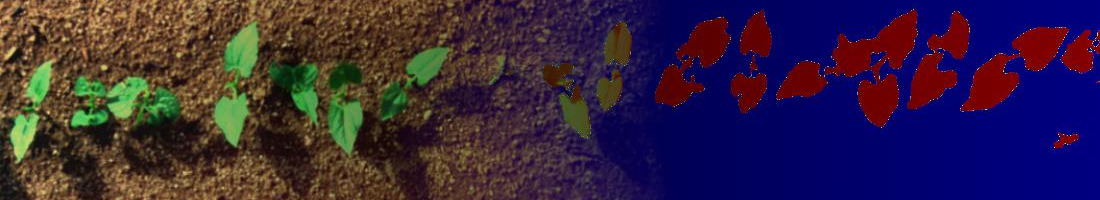
\includegraphics[width=\linewidth]{img/idx/graphical-gca}
	
	\paragraph{Authors} Jehan-Antoine Vayssade, Jean-Noël Paoli, Christelle Gée and Gawain Jones
	
	\paragraph{Publication} 09/06/2021 -- Remote Sensing Journal -- Volume 13 Issue 12 Pages 2261
	
	\paragraph{Abstract} The form of a remote sensing index is generally empirically defined, whether by choosing specific reflectance bands, equation forms or its coefficients. These spectral indices are used as preprocessing stage before object detection/classification. But no study seems to search for the best form through function approximation in order to optimize the classification and/or segmentation. The objective of this study is to develop a method to find the optimal index, using a statistical approach by gradient descent on different forms of generic equations. From six wavebands images, five equations have been tested, namely: linear, linear ratio, polynomial, universal function approximator and dense morphological. Few techniques in signal processing and image analysis are also deployed within a deep-learning framework. Performances of standard indices and DeepIndices were evaluated using two metrics, the dice (similar to f1-score) and the mean intersection over union (mIoU) scores. The study focuses on a specific multispectral camera used in near-field acquisition of soil and vegetation surfaces. These DeepIndices are built and compared to $89$ common vegetation indices using the same vegetation dataset and metrics. As an illustration the most used index for vegetation, NDVI (Normalized Difference Vegetation Indices) offers a mIoU score of \SI{63.98}{\percent} whereas our best models gives an analytic solution to reconstruct an index with a mIoU of \SI{82.19}{\percent}. This difference is significant enough to improve the segmentation and robustness of the index from various external factors, as well as the shape of detected elements.
	
	\paragraph{Keywords} image ; precision agriculture ; spectral indices ; multi-spectral ; deep-learning ; vegetation segmentation
    \vfill
	
	\newpage
	\section{Introduction}
	An important advance in the field of earth observation is the discovery of spectral indices, they have proved their effectiveness in surface description. Several studies have been conducted using remote sensing indices, often applied to a specific field of study like evaluations of vegetation cover, vigor, or growth dynamics \cite{SignificantVegetationIndices, ComparisonSentinel2, ReviewVegetationIndices, w13040547} for precision agriculture using multi-spectral sensors. Some spectral indices have been developed using RGB or HSV color space to detect vegetation from ground cameras \cite{LeeSegmentation, Milioto2017, HassaneinVegetation}. %, kumari2020grass}.
	Remote sensing indices {can also be used for other surfaces analysis like water, road, snow \cite{rs11232774} cloud \cite{ZHAI2018235} or shadow \cite{henrich2009development}.}
	
	There are two main problems with these indices. Firstly they are almost all empirically defined, although the selection of wavelengths comes from observation, like NDVI for vegetation indices. It is possible to obtain better spectral combinations or equations to characterize a surface with specific acquisitions parameters. It is important to optimize upstream the index, as the data transformation leads to a loss of essential information and features for classification \cite{Zhang2015}. Most studies have tried to optimize some parameters of existing indices. For example, an optimization of NDVI $(NIR-Red)/(NIR+Red)$ was proposed by \cite{gitelson2004wide} under the name of WDRVI (Wide Dynamic Range Vegetation Index) $(\alpha NIR - Red)/(\alpha NIR + Red)$. The author tested different values for $\alpha$ between 0 and 1. The ROC curve was used to determine the best coefficient for a given ground truth. Another optimized NDVI was designed and named EVI (Enhanced Vegetation Index). It takes into account the blue band for atmospheric resistance by including various parameters $G (NIR-Red) / (NIR + C_1 Red - C_2 Blue +L)$, where $G,L$ are respectively the gain factor and the canopy background adjustment, in addition the coefficients $C_1,C_2$ are used to compensate for the influence of clouds and shadows. Many other indices can be found in an online database of indices ({IDB}: \url{www.indexdatabase.de} accessed August 10, 2019) %Please add accessed date.
	 \cite{henrich2009development} including the choice of wavelengths and coefficients depending on the selected sensors or applications. But none of the presented indices are properly optimized. Thus, in the standard approach, the best index is determined by testing all available indices against the spectral bands of the selected sensor with a Pearson correlation between these indices and a ground truth \cite{Liu2017, Kokhan119808}. Furthermore, correlation is not the best estimator because it neither considers the class ratio nor the shape of the obtained segmentation and may again result in a non-optimal solution for a specific segmentation task. Finally, these indices are generally not robust because they are still very sensitive to shadows \cite{Zhang2015}. For vegetation, until recently, all of the referenced popular indices were man-made and used few spectral bands (usually NIR, red, sometimes blue or RedEdge).
	
	\newpage
	The second problem with standard indices is that they work with reflectance-calibrated data. Three calibration methods can be used in proximal-sensing. (i) The first method use an image taken before acquisition containing a color patch as a reference \cite{Yahui2019, rs11202428}, and is used for correction. The problem with this approach is that if the image is partially shaded, the calibration is only relevant on the non-shaded part. Moreover ideally the reference must be updated to reduce the interference of weather change on the spectrum measurement, which is not always possible since it's a human task. (ii) An other method is the use of an attached sunshine sensor \cite{gilliot:hal-02738181}, which also requires calibration but does not allow to correct a partially shaded image. (iii) The last method is the use of a controlled lighting environment \cite{Chebrolu2017, 8793974}, e.g., natural light is suppressed by a curtain and replaced by artificial lighting. All of these approaches are sometimes difficult to implement for automatic, outdoor use, and moreover in real time like detecting vegetation while a tractor is driving through a crop field.
	
	In recent years, machine learning algorithms have been increasingly used to improve the definition of presented indices in the first main problem. Some studies favor the use of multiple indices and advanced classification techniques (RandomForest, Boosting, DecisionTree, etc.) \cite{OLDELAND20101155, PENABARRAGAN20111301, NguyRobertson2012GreenLA, Shishir2018, w13040547, LU202142}. Another study has proposed to optimize the weights in an NDVI equation form based on a genetic algorithm \cite{GeneticKabiri} but does not optimize the equation forms. An other approach has been proposed to automatically construct a vegetation index using a genetic algorithm \cite{GeneticAlbarracin}. They optimize the equation forms by building a set of arithmetic graphs with mutations, crossovers and replications to change the shape of each equation during learning but it does not take into account the weights, since it's use calibrated data. Finally, with the emergence of deep learning, current studies try to adapt popular CNN architectures (UNet, AlexNet, etc.) to earth observation applications: \cite{rs10121946, gaetano:hal-01931435, 1.JRS.12.025010, Kussul2017DeepLC}. 
	
	However there is no study that optimize both the equation forms and spectral bands weights. The present study explicitly optimize both of them by looking for a form of remote sensing indices by learning weights in functions approximators. These functions approximators will then reconstruct any equation forms of the desired remote sensing index for a given acquisition system. 
	To solve the presented second problem, this study evaluates the functions approximators on an uncalibrated dataset containing various acquisition conditions. This is not a common approach but can be found in the literature \cite{Bajwa2002, Bareth2016}. This will lead to creating indices that do not require data calibration. The deep learning framework has been used as a general regression toolkit. Thus, several CNN function approximators architectures are proposed. DeepIndices is presented as a regression problem, which is totally new, as is the use of signal and image processing.
	
	\newpage
	\section{Material and Data}
	\label{sec:mat-data}
	
	
	\subsection{Instrument Details}
	The images were acquired with the Airphen (Hyphen, Avignon, France) six-band multi-spectral camera (Figure \ref{fig:camera}). This is a multi-spectral scientific camera developed by agronomists for agricultural applications. It can be integrated into different types of platforms such as drones, phenotyping robots, etc.
	
	\begin{figure}[H]
		\centering
		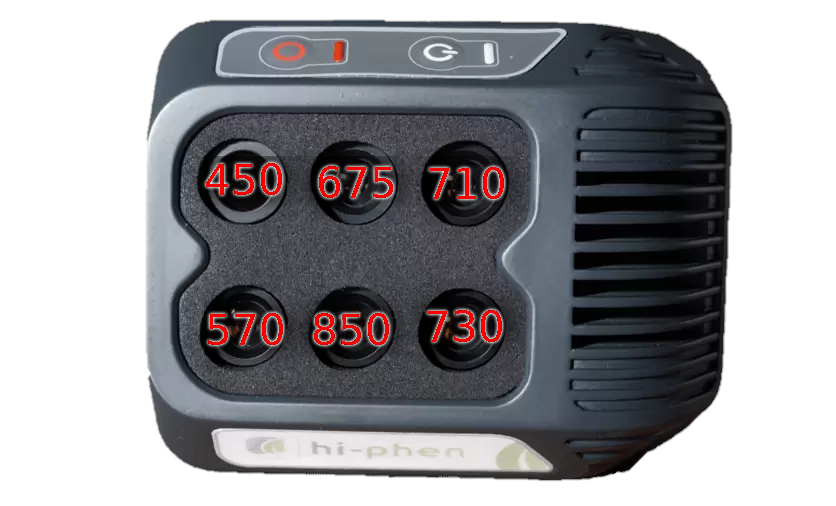
\includegraphics[height=3cm]{img/idx/airphen-detail4}
		\caption{AIRPHEN camera composed of 6 sensors}
		\label{fig:camera}
	\end{figure}
	
	
	The camera has been configured using the 450/570/675/710/730/850 nm bands with a 10 nm FWHM respectively denoted from $\lambda_{0}$ to $\lambda_{5}$. These spectral bands have been defined by a previous study \cite{Louargant2017} for crop/weed discrimination.
	The focal length of each lens is 8 mm. The raw resolutions for each spectral band is 1280  $\times$ 960 px with 12 bit precision. Finally, the camera is equipped with an internal GPS antenna.
	
	\subsection{Image Dataset}
	%Different type of acquisition have been characterized in order to propose different types of indices. Thus three ground truth have been defined to show the performances of the method is various field:
	
	%\paragraph{Ground truth to detect vegetation}
	The dataset were acquired on the site of INRAe in Montoldre (Allier, France) within the framework of the “RoSE challenge” founded by the French National Research Agency (ANR) and in Dijon (Burgundy, France) within the site of AgroSup Dijon. Images of bean and corn, containing various natural weeds (yarrows, amaranth, geranium, plantago, etc) and sowed ones (mustards, goosefoots, mayweed and ryegrass) with very distinct characteristics in terms of illumination (shadow, morning, evening, full sun, cloudy, rain, etc) were acquired in top-down view at 1.8 m from the ground. The Table \ref{tab:acquisition-source} synthesis the dataset.
	
	\begin{table}[H]
		\centering
        \rowcolors{0}{gray!10}{white}
		\begin{tabular}{|l|c|c|c|l|}
			\hline \textbf{Source}    & \textbf{Year} & \textbf{Corn} & \textbf{Bean} & \textbf{Illumination} \\ 
			\hline Dijon     & 2019 &  - & 9  & full sun, evening \\
			\hline Montoldre & 2019 & 20 & 22 & shadow, sunny, cloudy\\
			\hline Montoldre & 2020 & 18 & 22 & morning, cloudy, rainy\\ \hline
			\textbf{Total} & & 38 & 53 & =91 \\ 
			\hline
		\end{tabular}
		\caption{Acquisition sources and global illumination.}
		\label{tab:acquisition-source}
	\end{table}
	
	
	Manual annotation takes about 4 h per image to obtain the best quality of ground truth, which is necessary for use in regression algorithms. Thus the ground truth size is small and defined with very distinctive illumination condition. To simulate light variations effect on the  ground truth images a random brightness ($20\%$) and a random saturation ($5\%$) are added to each spectral band during the training phase. As illustration the Figure \ref{fig:culture-adventice} shows a false color reconstruction of corn crop in the field with various weeds and shadows on the corners of the image (not vignetting).
	
	\begin{figure}[H]
		\centering
		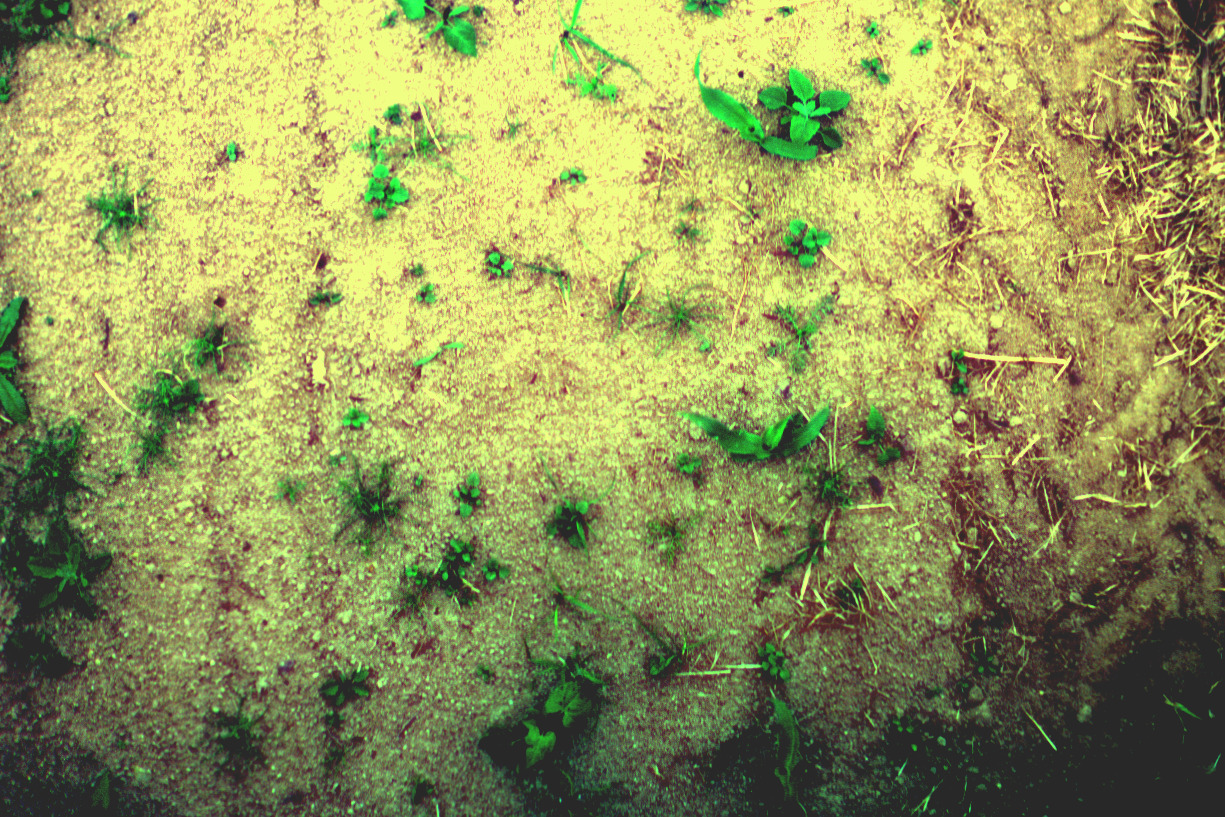
\includegraphics[width=0.3\linewidth]{img/idx/false}
		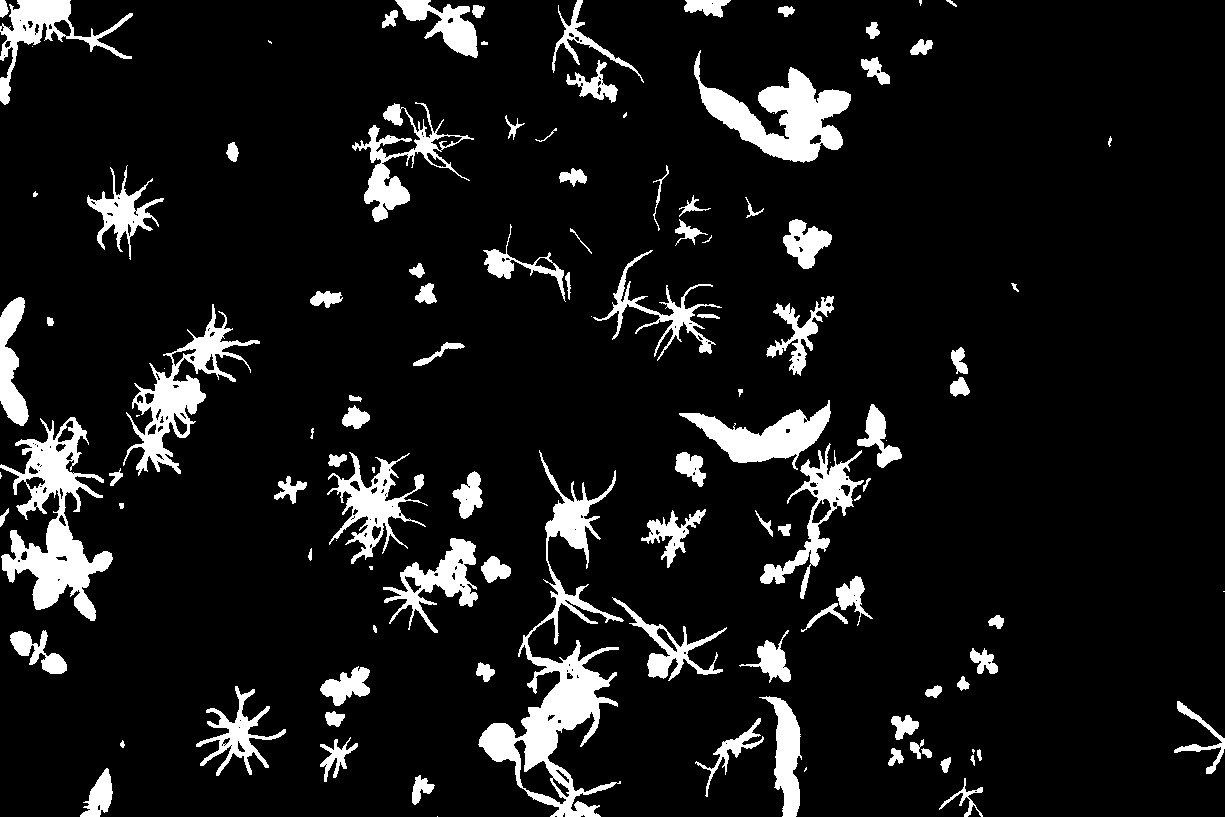
\includegraphics[width=0.3\linewidth]{img/idx/MASK}
		\caption{False color in the left and corresponding manual ground truth on the right.}
		\label{fig:culture-adventice}
	\end{figure}
	
	
	\subsection{Data Pre-Processing}
	
	\subsubsection{Images Registration} Due to the nature of the camera (Figure \ref{fig:camera}), a spectral band registration is required and performed with a registration method based on previous work \cite{vayssade:hal-02499730} (with a sub-pixel registration accuracy). The alignment is refined in two steps, with (i) a rough estimation of the affine correction and (ii) a perspective correction for the refinement and accuracy through the detection and matching of key points. The result shows that \textit{GoodFeatureToTrack} (GFTT) algorithm is the best key-point detector considering the $\lambda_{570}$ nm band as spectral reference for the registration. After the registration, all spectral images are cropped to $1200 \times 800$ px and concatenated to channel-wise denoted $\lambda$ where each dimension denoted $\lambda_d$ refers to each of the six spectral bands.
	
	\subsubsection{Images Normalization} Spectral bands inherently have a high noise associated with the CCD sensor, which is a potential problem during normalization \cite{7989768}. To overcome this effect, $1\%$ of the minimum and maximum signal is suppressed by calculating the quantiles, the signal is clipped on the given range and each band is rescaled in the interval $[0,1]$ using min-max normalization to obtain $\rho_d$:
	\begin{equation} \rho_d = 0 \leq \frac{\lambda_d-min(\lambda_d)}{max(\lambda_d)-min(\lambda_d)} \leq 1 \end{equation}
	
	The method also reduces the lighting variation. According to \cite{Blackburn2012} a little variation is observed in the spectral correction factors between clear and cloudy days. Thus, the correction has a limited impact on the scaling factor and should be managed by this equation. However, the displacement factor could not be estimated, thus the output images are not calibrated in reflectance.
	
	\subsubsection{Enriching Information} In order to enrich the pool of information, some spectral band transformations are added, which allow to take into account spatial gradients and spectral mixing \cite{Milioto2017} in the image. The choice is oriented towards seven important information in different respects:
	
	The standard deviation between spectral band, noted $\rho_{std}$ can help to detect the spectral mixture. For example between two different surface like ground and leave which have opposite spectral radiance the spectral mixing make a pixel with linear combination, thus the standard deviation tend to zero \cite{Louargant2017}.
	Three Gaussian derivatives on different orientations are computed $Gxx$, $Gxy$ and $Gyy$ over the standard deviation $\rho_{std}$ which give an important spatial information about the gradients breaks corresponding to the outer limits of surfaces. These Gaussian derivatives are computed with a fixed  $Sigma=1$.
	The Laplacian computed over the standard deviation $\rho_{std}$, the minimum and maximum eigenvalues of the Hessian matrix (obtained by Gaussian derivation $Gxx$, $Gxy$ and $Gyy$), also called ridge are included. These transformations sould improve the detection of fine elements \cite{LinVessel} such as monocotyledons for vegetation images.
	
	All these transformations are concatenated to the channel-wise normalized spectral band input and build the final input image. In total seven transformations are added to the six spectral images for a final image of 13 channels, which will probably help the convergence.
	
	\subsection{Training and Validation Datasets}
	The input dataset is composed by spectral images $\mathbf{I}$ of size $1200 \times 800 \times 13$ (or 6 if the ``Enriching information'' part is disabled) and a manual ground truth $\mathbf{p}$ of size $1200 \times 800 \times 1$  {where} $p \in \{0,1\}$. The desired output $\hat{p}$ is a probability vegetation map of size $1200 \times 800 \times 1$ where $\hat{p} \in [0,1]$. This input dataset is randomly split into two sub-sets respectively training (80\%) and validation (20\%). All random seed is fixed at the start-up to keep the same training/validation dataset across all trained models which help to compare them. Keeping the same random seed also results in the same starting point between different new runs, making results reproducible on the same hardware.%Is the bold in these equation necessary? Can we remove it?
	
	\section{Methodology}
	\label{sec:methodology}
	
	
	\subsection{Existing Spectral Indices}
	From the indices database, 89 vegetation indices have been identified (Table \ref{tab:fixed-veg-indices}) as compatible with the wavelengths used in this study (as near as possible), they will be tested and compared to the designed DeepIndices. Five forms of simple equations have been extracted from this database (a wide variety of indices are derived from these forms, generally a combination of 2 or 3 bands):
	
	\begin{eqnarray}
		\texttt{band reflectance} &=& \rho_i \label{eqn:band_reflectances} \\
		\texttt{two bands difference} &=& \rho_i - \rho_j \label{eqn:two_bands_difference} \\
		\texttt{two bands ratio} &=& \rho_i \div \rho_j  \label{eqn:two_bands_ratio} \\
		\texttt{normalized difference two bands} &=& (\rho_i - \rho_j) \div (\rho_i + \rho_j)  \label{eqn:normalized_difference_two_band} \\
		\texttt{normalized difference three bands} &=& (2\rho_i - \rho_j - \rho_k) \div (2\rho_i + \rho_j + \rho_k)  \label{eqn:normalized difference_three_band}
	\end{eqnarray}
	
	By analyzing these five equations we can synthesize them into two generic equations (Linear combination and Linear ratio) which take into account all spectral bands. Three other models can generalize any function: the polynomial fitting, the continuous function approximations by Taylor development, and the piecewise continuous function approximations trough morphological operators. These forms are interesting to optimize because they can approximate any function. This optimization will lead to automatically defining new indices (DeepIndices). The following subsections present these different models.
	
	\subsection{Deepindices: Baseline Models}
	\label{sec:gen-eqn}
	
	\subsubsection{Linear Combination} To synthesize Equations (\ref{eqn:band_reflectances}) and \eqref{eqn:two_bands_difference}, a simple linear equation such as $y = \sum_{d=0}^{N}{\alpha_d \rho_d}$ can be defined. This equation can be generalized to the 2D domain using a 2D convolution allowing consider the neighboring pixels. For a pixel at the position $[i,j]$ the convolution is defined by:
	\begin{equation} y[i,j] = \sum_{d=0}^{D} \sum_{h=0}^{N}\sum_{w=0}^{N}{\rho_d[i-N/2+h,j-N/2+w] \ast H[h,w,d]}  \end{equation}
	where $H$ defines neighborhood weights (corresponding to $\alpha_i$). $D$ is the number of dimensions (6 spectral bands + 5 transformations) and $N$ is the kernel size. The linear combination is given by $N=1, D=12$. The kernel weights are initialized by a truncated normal distribution centered on zero \cite{he_normal}, weights are updated during the training of the CNN trough back-propagation and unnecessary bands should be set to zero. The interesting part is that increasing the kernel size $N$ allows to take into account the neighborhood of a pixel and should estimate more accurately the spectral mixing \cite{Louargant2017}. Figure \ref{fig:linear} shows the corresponding network.
	
	\begin{figure}[H]
		\centering
		\tikzset{
	ppblock/.style={
		rectangle,
		minimum size=6mm,
		very thick,
		draw=black!50,
		text centered,
		font=\ttfamily,
		minimum width=8em,
		minimum height=6mm,
		top color=white,
	},
	%
	figure/.style={
		rectangle,
		rectangle split,
		rectangle split parts=2,
		very thick,
		draw=black!50,
		text centered,
		append after command={
			\pgfextra
			\fill[top color=#1, bottom color=#1]
			(\tikzlastnode.one west) 
			[rounded corners] |- (\tikzlastnode.north) -| (\tikzlastnode.one east) 
			[sharp corners]   |- (\tikzlastnode.one split) -| cycle;
			\fill[top color=white, bottom color=#1]
			(\tikzlastnode.two west) 
			[rounded corners] |- (\tikzlastnode.south) -| (\tikzlastnode.two east)  
			[sharp corners]   |- (\tikzlastnode.one split) -| cycle;
			\endpgfextra
		},
	},
    splitted/.style={
        rectangle,
        rectangle split,
        rectangle split horizontal,
        rectangle split parts=2,
        very thick,
        draw=black!50,
        text centered,
        append after command={
            \pgfextra
            \fill[top color=white, bottom color=#1]
            (\tikzlastnode.south)
            [rounded corners] -| (\tikzlastnode.west) |- (\tikzlastnode.one north)
            [sharp corners]   -| (\tikzlastnode.one split) |- cycle;
            \fill[top color=white, bottom color=#1]
            (\tikzlastnode.two south)
            [rounded corners] -| (\tikzlastnode.east) |- (\tikzlastnode.north)
            [sharp corners]   -| (\tikzlastnode.one split) |- cycle;
            \endpgfextra
        },
    },
	%
	static/.style={ppblock, bottom color={black!20}},
	nonterminal/.style={ppblock, bottom color={blue!30}},
	terminal/.style={ppblock, bottom color={green!20}},
	algorithm/.style={ppblock, bottom color={yellow!50}},
	error/.style={ppblock, bottom color={red!20}},
	type/.style={ppblock, bottom color={red!20}},
	loss/.style={ppblock, dashed, bottom color={black!20}, font=\itshape},
	%
	tiny/.style={
		rounded rectangle,
		very thick,
		draw=black!50,
		top color=white,
		bottom color=red!20,
        text centered,
		font=\ttfamily,
	},
    operator/.style = {
        circle,
        scale=0.6,
        draw=black!50,
        top color=white,
        bottom color=red!20,
        font=\boldmath,
    },
	%
	skip loop/.style={to path={-- ++(0,#1) -| (\tikztotarget)}}
}

\vspace{-1em}
\begin{tikzpicture}[
    >=stealth',thick,
    tip/.style={->,shorten >=0.007pt},
    every node/.style={scale=0.7},
]

\matrix[column sep=4mm, row sep=4mm, align=center] {
    % First row:
    \node (raw)    [terminal]      {Input \\ 1x1200x800xN};         &
    \node (conv1)  [nonterminal]   {Conv 1x1 \\ 1x1200x800x1};      &
    \node (out)    [terminal]      {Output \\ 1x1200x800x1};        \\
};

\begin{scope}[->,rounded corners=2mm]
  \draw[->]     (raw) -- (conv1);
  \draw[->]     (conv1) -- (out);
\end{scope}

\end{tikzpicture}
		\caption{Linear combination model.}
		\label{fig:linear}
	\end{figure}
	
	
	\subsubsection{Linear Ratio} To generalize Equations (\ref{eqn:two_bands_ratio})--(\ref{eqn:normalized difference_three_band}), a simple model based on the division of two linear combination is set. In the same way, this form is generalizable to the 2D domain and then corresponds to two 2D convolutions, one for the numerator, the other for the denominator. When the denominator is zero, the result is set to zero as well, to leverage the ``not a number'' output. The Figure \ref{fig:linear-ratio} shows the corresponding network.
	
	\begin{figure}[H]
		\centering
		\tikzset{
	ppblock/.style={
		rectangle,
		minimum size=6mm,
		very thick,
		draw=black!50,
		text centered,
		font=\ttfamily,
		minimum width=8em,
		minimum height=6mm,
		top color=white,
	},
	%
	figure/.style={
		rectangle,
		rectangle split,
		rectangle split parts=2,
		very thick,
		draw=black!50,
		text centered,
		append after command={
			\pgfextra
			\fill[top color=#1, bottom color=#1]
			(\tikzlastnode.one west) 
			[rounded corners] |- (\tikzlastnode.north) -| (\tikzlastnode.one east) 
			[sharp corners]   |- (\tikzlastnode.one split) -| cycle;
			\fill[top color=white, bottom color=#1]
			(\tikzlastnode.two west) 
			[rounded corners] |- (\tikzlastnode.south) -| (\tikzlastnode.two east)  
			[sharp corners]   |- (\tikzlastnode.one split) -| cycle;
			\endpgfextra
		},
	},
    splitted/.style={
        rectangle,
        rectangle split,
        rectangle split horizontal,
        rectangle split parts=2,
        very thick,
        draw=black!50,
        text centered,
        append after command={
            \pgfextra
            \fill[top color=white, bottom color=#1]
            (\tikzlastnode.south)
            [rounded corners] -| (\tikzlastnode.west) |- (\tikzlastnode.one north)
            [sharp corners]   -| (\tikzlastnode.one split) |- cycle;
            \fill[top color=white, bottom color=#1]
            (\tikzlastnode.two south)
            [rounded corners] -| (\tikzlastnode.east) |- (\tikzlastnode.north)
            [sharp corners]   -| (\tikzlastnode.one split) |- cycle;
            \endpgfextra
        },
    },
	%
	static/.style={ppblock, bottom color={black!20}},
	nonterminal/.style={ppblock, bottom color={blue!30}},
	terminal/.style={ppblock, bottom color={green!20}},
	algorithm/.style={ppblock, bottom color={yellow!50}},
	error/.style={ppblock, bottom color={red!20}},
	type/.style={ppblock, bottom color={red!20}},
	loss/.style={ppblock, dashed, bottom color={black!20}, font=\itshape},
	%
	tiny/.style={
		rounded rectangle,
		very thick,
		draw=black!50,
		top color=white,
		bottom color=red!20,
        text centered,
		font=\ttfamily,
	},
    operator/.style = {
        circle,
        scale=0.6,
        draw=black!50,
        top color=white,
        bottom color=red!20,
        font=\boldmath,
    },
	%
	skip loop/.style={to path={-- ++(0,#1) -| (\tikztotarget)}}
}

\vspace{-1em}
\begin{tikzpicture}[
		>=stealth',thick,
		tip/.style={->,shorten >=0.007pt},
		every node/.style={scale=0.7},
	]
	\matrix[column sep=4mm, row sep=4mm, align=center] {
		\node (raw)    [terminal]      {Input \\ 1x1200x800xN};         &
		\node (conv1)  [nonterminal]   {Conv 1x1 \\ 1x1200x800x1};      &
		\node (div)    [static]      {DivNaN \\ 1x1200x800x1};        &
		\node (out)    [terminal]      {Output \\ 1x1200x800x1};        \\
		& \node (conv2)  [nonterminal]   {Conv 1x1 \\ 1x1200x800x1}; & \\
	};
	
	\begin{scope}[->,rounded corners=2mm]
	\draw[->]     (raw) -- (conv1);
	\draw[->]     (raw) |- (conv2);
	\draw[->]     (conv1) -- (div);
	\draw[->]     (conv2) -| (div);
	\draw[->]     (div) -- (out);
	\end{scope}

\end{tikzpicture}
		\caption{ {Linear} ratio model.}
		\label{fig:linear-ratio}
	\end{figure}%We kindly request authors to provide figures and schemes at a sufficiently high resolution (min. 600 pixels width, 300 dpi), in order to convert a clear PDF document with high quality. Therefore, please kindly provide sharper figures.
	
	\subsubsection{Polynomial} According to the Stone-Weierstrass theorem any continuous function defined on a segment can be uniformly approximated by a polynomial function. Thus all forms of color indices can be approximated by a polynomial $y = \sum_{d=0}^{N}{\alpha_d \rho_d}^{\delta_d}$ of degree $N$. Setting the degree is a difficult task which may imply under-fitting or over-fitting. In addition un-stability can be caused by near-zero $\delta_d$. But since the segment is restricted to the domain $[0,1]$ the Bernstein polynomials are a common demonstration and the equation can be wrote as a weighted sum of Bernstein basis polynomials $B_{N,i} = (1-\rho)^{i} \rho^{N-i}$ which are more stable during the training. Moreover Bernstein Neural Network can solve partially differentiable equations \cite{Sun2018SolvingPD}. For implementation reasons, two different layers are defined in the network (visible in the Figure \ref{fig:polynomial}). One for the Bernstein expansion limited to $B_{11,11}$ which takes the input image and produces different Bernstein basis polynomial, then each Bernstein basis is concatenated to the channel-wise and the linear combination is defined by a \mbox{2D convolution.}
	% An additional hyperparameter are used for t
	
	\begin{figure}[H]
		\centering
		\tikzset{
	ppblock/.style={
		rectangle,
		minimum size=6mm,
		very thick,
		draw=black!50,
		text centered,
		font=\ttfamily,
		minimum width=8em,
		minimum height=6mm,
		top color=white,
	},
	%
	figure/.style={
		rectangle,
		rectangle split,
		rectangle split parts=2,
		very thick,
		draw=black!50,
		text centered,
		append after command={
			\pgfextra
			\fill[top color=#1, bottom color=#1]
			(\tikzlastnode.one west) 
			[rounded corners] |- (\tikzlastnode.north) -| (\tikzlastnode.one east) 
			[sharp corners]   |- (\tikzlastnode.one split) -| cycle;
			\fill[top color=white, bottom color=#1]
			(\tikzlastnode.two west) 
			[rounded corners] |- (\tikzlastnode.south) -| (\tikzlastnode.two east)  
			[sharp corners]   |- (\tikzlastnode.one split) -| cycle;
			\endpgfextra
		},
	},
    splitted/.style={
        rectangle,
        rectangle split,
        rectangle split horizontal,
        rectangle split parts=2,
        very thick,
        draw=black!50,
        text centered,
        append after command={
            \pgfextra
            \fill[top color=white, bottom color=#1]
            (\tikzlastnode.south)
            [rounded corners] -| (\tikzlastnode.west) |- (\tikzlastnode.one north)
            [sharp corners]   -| (\tikzlastnode.one split) |- cycle;
            \fill[top color=white, bottom color=#1]
            (\tikzlastnode.two south)
            [rounded corners] -| (\tikzlastnode.east) |- (\tikzlastnode.north)
            [sharp corners]   -| (\tikzlastnode.one split) |- cycle;
            \endpgfextra
        },
    },
	%
	static/.style={ppblock, bottom color={black!20}},
	nonterminal/.style={ppblock, bottom color={blue!30}},
	terminal/.style={ppblock, bottom color={green!20}},
	algorithm/.style={ppblock, bottom color={yellow!50}},
	error/.style={ppblock, bottom color={red!20}},
	type/.style={ppblock, bottom color={red!20}},
	loss/.style={ppblock, dashed, bottom color={black!20}, font=\itshape},
	%
	tiny/.style={
		rounded rectangle,
		very thick,
		draw=black!50,
		top color=white,
		bottom color=red!20,
        text centered,
		font=\ttfamily,
	},
    operator/.style = {
        circle,
        scale=0.6,
        draw=black!50,
        top color=white,
        bottom color=red!20,
        font=\boldmath,
    },
	%
	skip loop/.style={to path={-- ++(0,#1) -| (\tikztotarget)}}
}

\vspace{-1em}
\begin{tikzpicture}[
		>=stealth',thick,
		tip/.style={->,shorten >=0.007pt},
		every node/.style={scale=0.7},
	]
	\matrix[column sep=4mm, row sep=4mm, align=center] {
		& \node (conv1)  [static]   {$X^3$ \\ 1x1200x800xN}; & \\
		\node (raw)    [terminal]      {Input \\ 1x1200x800xN};         &
		\node (conv2)  [static]   {$X^2(1-X)$ \\ 1x1200x800xN};         &
		\node (div)    [nonterminal]      {Conv 1x1 \\ 1x1200x800x1};        &
		\node (out)    [terminal]      {Output \\ 1x1200x800x1};        \\
		& \node (conv3)  [static]   {$X(1-X)^2$ \\ 1x1200x800xN}; & \\
		& \node (conv4)  [static]   {$(1-X)^3$ \\ 1x1200x800xN}; & \\
	};
	
	\begin{scope}[->,rounded corners=2mm]
		\draw[->]     (raw) |- (conv1);
		\draw[->]     (raw) -- (conv2);
		\draw[->]     (raw) |- (conv3);
		\draw[->]     (raw) |- (conv4);
		\draw[->]     (conv1) -| (div);
		\draw[->]     (conv2) -- (div);
		\draw[->]     (conv3) -| (div);
		\draw[->]     (conv4) -| (div);
		\draw[->]     (div) -- (out);
	\end{scope}

\end{tikzpicture}
		\caption{ {Polynomial} model with Bernstein expansions between $B_{4,1}$ and $B_{4,4}$.}
		\label{fig:polynomial}
	\end{figure}%We kindly request authors to provide figures and schemes at a sufficiently high resolution (min. 600 pixels width, 300 dpi), in order to convert a clear PDF document with high quality. Therefore, please kindly provide sharper figures. This figure is not mentioned in maintext, please confirm.
	
	
	% http://alexadam.ca/ml/2017/08/10/unversal-approximation-theorem-part-1.html
	\subsubsection{Universal Function Approximation} The Gaussian color space model proposed by \cite{Geusebroek2000} shows that the spatio-spectral energy distribution of the incident light $E$ is the weighted integration of the spectrum $\rho_d$ denoted $E(\rho_d)$. Where $E$ can be described as a Taylor series and the energy function is convolved by different derivatives of a Gaussian kernel or structured receptive fields \cite{ReceptiveField}. This important point shows that Taylor expansions can decompose any function $f(x)$, especially for color decomposition and remapping, into :
	
	\begin{equation} f(x) = f(0) + f'(x) x + \frac{1}{2!} f''(x) x^2 + \frac{1}{3!} f'''(x) x^3 + o(x^3) \end{equation}
	%\begin{equation} f(x) = \sum_{n=0}^{\inf} \frac{f^n(a)}{n!}(x-a)^n \end{equation}
	
	Here, the signature of the incident energies distribution of a remote sensing index associated to a surface can be reconstructed. An approach to learn this form of development is proposed by \cite{DenseNet} which is commonly called DenseNet and then corresponds to the sum of the concatenation of the signal and these spatio-spectral derivatives
	
	\begin{equation} \mathbf{x} \to \left [\mathbf{x}, f_1(\mathbf{x}), f_2(\mathbf{x}, f_1(\mathbf{x})), \ldots\right] \end{equation}
	
	Various convolutions allow to learn receptive fields and derivatives in spectral domain when the kernel size $k$ is 1, and in spatio-spectral domain when $k$ is higher. Batch-Normalization are used to reduces the covariate shift across convolution output by re-scaling it and speed up the convergence. Finally the Sigmoid activation function is used and defined by
	
	\begin{equation} Sigmoid(x) = \frac{1}{1+e^{-x}} \end{equation}
	
	Sigmoid function allows to learn more complex structures and non-linearity of the reconstructed function. 
	The number of derivative and receptive field are configurable with two parameters. The $depth$ which corresponds to the number of layers in the network. And the $width$ which refers to the number of outputs for each convolution. By default, the $depth$ is fixed to $3$ and the $width$ is fixed to $5$. The Figure \ref{fig:universal-function-approximator} shows the corresponding universal function approximator network.
	
	%Formally the energies distribution of the wavelength can be wrote $\rho_d$ at a spatial position $[i,j]$ as $E(\rho_d, i, j) = $ ...
	%The relation between the sigmoid function and the Gaussian can be shown by derivation of the sigmoid function to achieve an approximate Gaussian \cite{sigmoid2gaussian}.
	%Due to the fact the $\rho$ is discretized and integrated on different images, the energies distribution is split along all spectral band and $E(\rho) = \sum_{d=0}^{N} E(\rho_d)$.
	%Thus the
	
	%http://www.wikiwand.com/en/Universal_approximation_theorem: The 'dual' versions of the theorem consider networks of bounded width and arbitrary depth. A variant of the universal approximation theorem was proved for the arbitrary depth case by Zhou Lu et all in 2017.[6] They showed that networks of width n+4 with ReLU activation functions can approximate any Lebesgue integrable function on n-dimensional input space with respect to L^{1} distance if network depth is allowed to grow.
	
	% https://hackernoon.com/illustrative-proof-of-universal-approximation-theorem-5845c02822f6
	
	\begin{figure}[H]
		\centering
		\tikzset{
	ppblock/.style={
		rectangle,
		minimum size=6mm,
		very thick,
		draw=black!50,
		text centered,
		font=\ttfamily,
		minimum width=8em,
		minimum height=6mm,
		top color=white,
	},
	%
	figure/.style={
		rectangle,
		rectangle split,
		rectangle split parts=2,
		very thick,
		draw=black!50,
		text centered,
		append after command={
			\pgfextra
			\fill[top color=#1, bottom color=#1]
			(\tikzlastnode.one west) 
			[rounded corners] |- (\tikzlastnode.north) -| (\tikzlastnode.one east) 
			[sharp corners]   |- (\tikzlastnode.one split) -| cycle;
			\fill[top color=white, bottom color=#1]
			(\tikzlastnode.two west) 
			[rounded corners] |- (\tikzlastnode.south) -| (\tikzlastnode.two east)  
			[sharp corners]   |- (\tikzlastnode.one split) -| cycle;
			\endpgfextra
		},
	},
    splitted/.style={
        rectangle,
        rectangle split,
        rectangle split horizontal,
        rectangle split parts=2,
        very thick,
        draw=black!50,
        text centered,
        append after command={
            \pgfextra
            \fill[top color=white, bottom color=#1]
            (\tikzlastnode.south)
            [rounded corners] -| (\tikzlastnode.west) |- (\tikzlastnode.one north)
            [sharp corners]   -| (\tikzlastnode.one split) |- cycle;
            \fill[top color=white, bottom color=#1]
            (\tikzlastnode.two south)
            [rounded corners] -| (\tikzlastnode.east) |- (\tikzlastnode.north)
            [sharp corners]   -| (\tikzlastnode.one split) |- cycle;
            \endpgfextra
        },
    },
	%
	static/.style={ppblock, bottom color={black!20}},
	nonterminal/.style={ppblock, bottom color={blue!30}},
	terminal/.style={ppblock, bottom color={green!20}},
	algorithm/.style={ppblock, bottom color={yellow!50}},
	error/.style={ppblock, bottom color={red!20}},
	type/.style={ppblock, bottom color={red!20}},
	loss/.style={ppblock, dashed, bottom color={black!20}, font=\itshape},
	%
	tiny/.style={
		rounded rectangle,
		very thick,
		draw=black!50,
		top color=white,
		bottom color=red!20,
        text centered,
		font=\ttfamily,
	},
    operator/.style = {
        circle,
        scale=0.6,
        draw=black!50,
        top color=white,
        bottom color=red!20,
        font=\boldmath,
    },
	%
	skip loop/.style={to path={-- ++(0,#1) -| (\tikztotarget)}}
}

\vspace{-1em}
\begin{tikzpicture}[
>=stealth',thick,
tip/.style={->,shorten >=0.007pt},
every node/.style={scale=0.7},
]
\matrix[column sep=4mm, row sep=4mm, align=center] {
	% first line
	\node (raw)    [terminal]      {Input \\ 1200x800xN};         &
	\node (conv1)  [nonterminal]   {Conv 1x1 \\ 1200x800x5};      &
	\node (bn1)    [static]        {BatchNorm};     &
	\node (sig1)   [static]        {Sigmoid};       &
	\node (p1)     [operator]      {$\cup$};                             \\
	% second line
	& % empty
	\node (conv2)  [nonterminal]   {Conv 1x1 \\ 1200x800x5};      &
	\node (bn2)    [static]        {BatchNorm};     &
	\node (sig2)   [static]        {Sigmoid};       &
	\node (p2)     [operator]      {$\cup$};                             \\
	% third line
	& % empty
	\node (conv3)  [nonterminal]   {Conv 1x1 \\ 1200x800x5};      &
	\node (bn3)    [static]        {BatchNorm};     &
	\node (sig3)   [static]        {Sigmoid};       &
	\node (p3)     [operator]      {$\cup$};                           &
	\node (out)    [terminal]      {Output \\ 1200x800x1};        \\
};

\begin{scope}[->,rounded corners=2mm]
\draw[->]     (raw) -- (conv1);
\draw[->]     (conv1) -- (bn1);
\draw[->]     (bn1) -- (sig1);
\draw[->]     (sig1) -- (p1);

\draw[->]     (p1.south) to [in=45,out=-90, looseness=0.3] (conv2.north);
\draw[->]     (conv2) -- (bn2);
\draw[->]     (bn2) -- (sig2);
\draw[->]     (sig2) -- (p2);

\draw[->]     (p2.south) to [in=45,out=-90, looseness=0.3] (conv3.north);
\draw[->]     (conv3) -- (bn3);
\draw[->]     (bn3) -- (sig3);
\draw[->]     (sig3) -- (p3);
\draw[->]     (p3) -- (out);


\draw[->]     (raw.north) to [in=135,out=45, looseness=0.3] (p1.north);
\draw[->]     (p1) -- (p2);
\draw[->]     (p2) -- (p3);
\end{scope}

\end{tikzpicture}
		\caption{ {Universal} function approximation model (depth = 3, width = 5).}
		\label{fig:universal-function-approximator}
	\end{figure}%We kindly request authors to provide figures and schemes at a sufficiently high resolution (min. 600 pixels width, 300 dpi), in order to convert a clear PDF document with high quality. Therefore, please kindly provide sharper figures.
	
	
	\subsubsection{Dense Morphological Function Approximation} As for the Taylor series, an approximation of any piecewise continuous function can be established by morphological operators such as dilatation and erosion \cite{DenseMorpho}, respectively denoted $\rho \oplus s$ and $\rho \ominus s$ where $s$ are the corresponding erosion or dilatation coefficients. Several erosion and dilation are defined for each spectral band $i$, then the expanded layer is defined as the channel concatenation of $ z_i^{+}$ and in the same way for the erosion layer via $z_i^{-}$. Both are defined by
	\begin{eqnarray}
	z_i^{+} = \rho \oplus s_i = \max_k(\rho_k - s_{k,i}, 0) \\
	z_i^{-} = \rho \ominus s_i = \max_k(s_{k,i} - \rho_k, 0)
	\end{eqnarray}
	
	To obtain the output $I = \sum_{i=0}^{N}{z_i^{+}w_i^{+}} + \sum_{i=0}^{N}{z_i^{-}w_i^{-}}$ of which the $w_i^{+}$ and the $w_i^{-}$ are the linear combination coefficients obtained by a 2D convolution. We chose to set the number of dilation and erosion neurons at 6. The Figure \ref{fig:dense-morphological} shows the corresponding network.
	
	\begin{figure}[H]
		\centering
		\tikzset{
	ppblock/.style={
		rectangle,
		minimum size=6mm,
		very thick,
		draw=black!50,
		text centered,
		font=\ttfamily,
		minimum width=8em,
		minimum height=6mm,
		top color=white,
	},
	%
	figure/.style={
		rectangle,
		rectangle split,
		rectangle split parts=2,
		very thick,
		draw=black!50,
		text centered,
		append after command={
			\pgfextra
			\fill[top color=#1, bottom color=#1]
			(\tikzlastnode.one west) 
			[rounded corners] |- (\tikzlastnode.north) -| (\tikzlastnode.one east) 
			[sharp corners]   |- (\tikzlastnode.one split) -| cycle;
			\fill[top color=white, bottom color=#1]
			(\tikzlastnode.two west) 
			[rounded corners] |- (\tikzlastnode.south) -| (\tikzlastnode.two east)  
			[sharp corners]   |- (\tikzlastnode.one split) -| cycle;
			\endpgfextra
		},
	},
    splitted/.style={
        rectangle,
        rectangle split,
        rectangle split horizontal,
        rectangle split parts=2,
        very thick,
        draw=black!50,
        text centered,
        append after command={
            \pgfextra
            \fill[top color=white, bottom color=#1]
            (\tikzlastnode.south)
            [rounded corners] -| (\tikzlastnode.west) |- (\tikzlastnode.one north)
            [sharp corners]   -| (\tikzlastnode.one split) |- cycle;
            \fill[top color=white, bottom color=#1]
            (\tikzlastnode.two south)
            [rounded corners] -| (\tikzlastnode.east) |- (\tikzlastnode.north)
            [sharp corners]   -| (\tikzlastnode.one split) |- cycle;
            \endpgfextra
        },
    },
	%
	static/.style={ppblock, bottom color={black!20}},
	nonterminal/.style={ppblock, bottom color={blue!30}},
	terminal/.style={ppblock, bottom color={green!20}},
	algorithm/.style={ppblock, bottom color={yellow!50}},
	error/.style={ppblock, bottom color={red!20}},
	type/.style={ppblock, bottom color={red!20}},
	loss/.style={ppblock, dashed, bottom color={black!20}, font=\itshape},
	%
	tiny/.style={
		rounded rectangle,
		very thick,
		draw=black!50,
		top color=white,
		bottom color=red!20,
        text centered,
		font=\ttfamily,
	},
    operator/.style = {
        circle,
        scale=0.6,
        draw=black!50,
        top color=white,
        bottom color=red!20,
        font=\boldmath,
    },
	%
	skip loop/.style={to path={-- ++(0,#1) -| (\tikztotarget)}}
}

\vspace{-1em}
\begin{tikzpicture}[
>=stealth',thick,
tip/.style={->,shorten >=0.007pt},
every node/.style={scale=0.7},
]
\matrix[column sep=4mm, row sep=4mm, align=center] {
	& \node ()     [nonterminal, xshift=-5, yshift=-5]  {Erosion \\ 1200x800xN};
	\node (ero1)   [nonterminal]  {Erosion \\ 1200x800xN};
	& \node (p1)   [operator] {$\times$}; \\
	%
	\node (raw)    [terminal]      {Input \\ 1200x800xN};         &
	\node ()       [nonterminal, xshift=-5, yshift=-5]    {Dilatation \\ 1200x800xN};
	\node (dil1)   [nonterminal]    {Dilatation \\ 1200x800xN};       &
	\node (p2)     [operator] {$\cup$}; &
	\node (conv1)  [nonterminal]   {Conv 1x1 \\ 1200x800x1};        &
	\node (out)    [terminal]      {Output \\ 1200x800x1};        \\
};

\begin{scope}[->,rounded corners=2mm]
	\draw[->]     (raw) -- (dil1);
	\draw[->]     (raw) -- (ero1.south west);
	\draw[->]     (dil1.north east) -- (p1);
	\draw[->]     (ero1) -- (p1);
	\draw[->]     (dil1) -- (p2);
	\draw[->]     (ero1.south east) -- (p2);
	\draw[->]     (p1) -- (p2);
	\draw[->]     (p2) -- (conv1);
	\draw[->]     (conv1) -- (out);
\end{scope}

\end{tikzpicture}
		\caption{ {Dense}-morphological model.}
		\label{fig:dense-morphological}
	\end{figure}
	
	\subsection{Enhancing Baseline Models}
	
	\subsubsection{Input Band Filter (IBF)} To remove parts of the signal that may be dispensable, the addition of a low-pass, high-pass and band-pass filter upstream of the network are studied. A good example is provided by vegetation indices, only the high values in the green and near infra-red, and the low values in the red and blue characterize the vegetation.
	
    \newpage
	This is the principle of the NDVI index. Due to the internal structure, the leaves reflect a lot of light in the near infrared, which is in sharp contrast to most non-vegetable surfaces. When the plant is dehydrated or stressed, the spongy layer collapse and the leaves reflect less light in the near-infrared, reaching red values in the visible range \cite{joshi2020revolution}. Thus, the mathematical combination of these two signals can help to differentiate plants from non-plant objects and healthy plants from diseased plants. However, this index is {then less interesting when detecting only vegetation and is strongly influenced by shade or heat.}
	
	We will therefore add a filter in the previous equations to remove undesirable spectral energies of each $\rho_d$ by using two thresholds a and b, which will also be learned. If it turns out that the whole signal is interesting, these two parameters will not change and their values will be a=0 and b=1. To apply the low-pass filter the equation $z = \max(\rho-a,0) \div (1-a)$ is used and thus allows to suppress low values. For the high-pass filter the equation $w = \max(b-\rho,0) \div b$ is applied to suppress high values. The band-pass filter it's the product of low and high-pass filters $y = z*x$. The output layer is the concatenation in the channel-wise of the input images, the low-pass, the high-pass and the band-pass filter which produce $4  \times 13=52$ channels. Finally to reduce the output data for the rest of the network, a bottleneck is inserted using a convolution layer, and generate a new image with 6 channels. This image is used by the rest of the network defined previously in Section \ref{sec:gen-eqn}. The Figure \ref{fig:input-band-filter} shows the corresponding module inserted upstream of the network.
	
	\begin{figure}[H]
		\centering
		\tikzset{
	ppblock/.style={
		rectangle,
		minimum size=6mm,
		very thick,
		draw=black!50,
		text centered,
		font=\ttfamily,
		minimum width=8em,
		minimum height=6mm,
		top color=white,
	},
	%
	figure/.style={
		rectangle,
		rectangle split,
		rectangle split parts=2,
		very thick,
		draw=black!50,
		text centered,
		append after command={
			\pgfextra
			\fill[top color=#1, bottom color=#1]
			(\tikzlastnode.one west) 
			[rounded corners] |- (\tikzlastnode.north) -| (\tikzlastnode.one east) 
			[sharp corners]   |- (\tikzlastnode.one split) -| cycle;
			\fill[top color=white, bottom color=#1]
			(\tikzlastnode.two west) 
			[rounded corners] |- (\tikzlastnode.south) -| (\tikzlastnode.two east)  
			[sharp corners]   |- (\tikzlastnode.one split) -| cycle;
			\endpgfextra
		},
	},
    splitted/.style={
        rectangle,
        rectangle split,
        rectangle split horizontal,
        rectangle split parts=2,
        very thick,
        draw=black!50,
        text centered,
        append after command={
            \pgfextra
            \fill[top color=white, bottom color=#1]
            (\tikzlastnode.south)
            [rounded corners] -| (\tikzlastnode.west) |- (\tikzlastnode.one north)
            [sharp corners]   -| (\tikzlastnode.one split) |- cycle;
            \fill[top color=white, bottom color=#1]
            (\tikzlastnode.two south)
            [rounded corners] -| (\tikzlastnode.east) |- (\tikzlastnode.north)
            [sharp corners]   -| (\tikzlastnode.one split) |- cycle;
            \endpgfextra
        },
    },
	%
	static/.style={ppblock, bottom color={black!20}},
	nonterminal/.style={ppblock, bottom color={blue!30}},
	terminal/.style={ppblock, bottom color={green!20}},
	algorithm/.style={ppblock, bottom color={yellow!50}},
	error/.style={ppblock, bottom color={red!20}},
	type/.style={ppblock, bottom color={red!20}},
	loss/.style={ppblock, dashed, bottom color={black!20}, font=\itshape},
	%
	tiny/.style={
		rounded rectangle,
		very thick,
		draw=black!50,
		top color=white,
		bottom color=red!20,
        text centered,
		font=\ttfamily,
	},
    operator/.style = {
        circle,
        scale=0.6,
        draw=black!50,
        top color=white,
        bottom color=red!20,
        font=\boldmath,
    },
	%
	skip loop/.style={to path={-- ++(0,#1) -| (\tikztotarget)}}
}

\vspace{-2em}
\begin{tikzpicture}[
    >=stealth',thick,
    tip/.style={->,shorten >=0.007pt},
    every node/.style={scale=0.7},
]
\matrix[column sep=4mm, row sep=4mm, align=center] {
	& \node (ero1) [nonterminal]  {$max(x-a)$ \\ 1200x800xN};
	& \node (p1)   [operator] {$\times$}; \\
	%
	\node (raw)    [terminal]      {Input \\ 1200x800xN};         &
	\node (dil1)   [nonterminal]    {$min(a-x)$ \\ 1200x800xN};       &
	\node (p2)     [operator] {$\cup$}; &
	\node (conv1)  [nonterminal]   {Conv 1x1 \\ 1200x800x1};        &
	\node (out)    [terminal]      {Output \\ 1200x800x1};        \\
	& \coordinate (p3);        \\
};

\begin{scope}[->,rounded corners=2mm]
    \draw[->]     (raw) -- (dil1);
    \draw[->]     (raw) -- (ero1.south west);
    \draw[->]     (dil1.north east) -- (p1);
    \draw[->]     (ero1) -- (p1);
    \draw[->]     (dil1) -- (p2);
    \draw[->]     (ero1.south east) -- (p2);
    \draw[->]     (raw.south) |- (p3) -| (p2.south);
    \draw[->]     (p1) -- (p2);
    \draw[->]     (p2) -- (conv1);
    \draw[->]     (conv1) -- (out);
\end{scope}

\end{tikzpicture}
		\caption{ {Input} Band Filter inserted at the beginning of the model.}
		\label{fig:input-band-filter}
	\end{figure}
	
	\subsubsection{Spatial Pyramid Refinement Block (SPRB)} To take into account different scales in the image, the addition of a ``Spatial Pyramid Refinement Block'' at the downstream part of the network is studied. \cite{SPRBWei} showed that fusing the low to high-level features improved the segmentation task. It consists in the sum of different 2D convolutions whose core sizes have been set to 3, 5, 7 and 9. The results of all convolutions are concatenated and the final image output is given by a 2D convolution. The Figure \ref{fig:spatial-refinement-block} shows the corresponding module inserted downstream of the network.
	
	\begin{figure}[H]
		\centering
		\tikzset{
	ppblock/.style={
		rectangle,
		minimum size=6mm,
		very thick,
		draw=black!50,
		text centered,
		font=\ttfamily,
		minimum width=8em,
		minimum height=6mm,
		top color=white,
	},
	%
	figure/.style={
		rectangle,
		rectangle split,
		rectangle split parts=2,
		very thick,
		draw=black!50,
		text centered,
		append after command={
			\pgfextra
			\fill[top color=#1, bottom color=#1]
			(\tikzlastnode.one west) 
			[rounded corners] |- (\tikzlastnode.north) -| (\tikzlastnode.one east) 
			[sharp corners]   |- (\tikzlastnode.one split) -| cycle;
			\fill[top color=white, bottom color=#1]
			(\tikzlastnode.two west) 
			[rounded corners] |- (\tikzlastnode.south) -| (\tikzlastnode.two east)  
			[sharp corners]   |- (\tikzlastnode.one split) -| cycle;
			\endpgfextra
		},
	},
    splitted/.style={
        rectangle,
        rectangle split,
        rectangle split horizontal,
        rectangle split parts=2,
        very thick,
        draw=black!50,
        text centered,
        append after command={
            \pgfextra
            \fill[top color=white, bottom color=#1]
            (\tikzlastnode.south)
            [rounded corners] -| (\tikzlastnode.west) |- (\tikzlastnode.one north)
            [sharp corners]   -| (\tikzlastnode.one split) |- cycle;
            \fill[top color=white, bottom color=#1]
            (\tikzlastnode.two south)
            [rounded corners] -| (\tikzlastnode.east) |- (\tikzlastnode.north)
            [sharp corners]   -| (\tikzlastnode.one split) |- cycle;
            \endpgfextra
        },
    },
	%
	static/.style={ppblock, bottom color={black!20}},
	nonterminal/.style={ppblock, bottom color={blue!30}},
	terminal/.style={ppblock, bottom color={green!20}},
	algorithm/.style={ppblock, bottom color={yellow!50}},
	error/.style={ppblock, bottom color={red!20}},
	type/.style={ppblock, bottom color={red!20}},
	loss/.style={ppblock, dashed, bottom color={black!20}, font=\itshape},
	%
	tiny/.style={
		rounded rectangle,
		very thick,
		draw=black!50,
		top color=white,
		bottom color=red!20,
        text centered,
		font=\ttfamily,
	},
    operator/.style = {
        circle,
        scale=0.6,
        draw=black!50,
        top color=white,
        bottom color=red!20,
        font=\boldmath,
    },
	%
	skip loop/.style={to path={-- ++(0,#1) -| (\tikztotarget)}}
}

\vspace{-1em}
\begin{tikzpicture}[
        >=stealth',thick,
        tip/.style={->,shorten >=0.007pt},
        every node/.style={scale=0.7},
    ]
	\matrix[column sep=4mm, row sep=4mm, align=center] {
		& \coordinate (p1); & \\
		& \node (conv1)  [nonterminal] {Conv 3x3 \\ 1200x800x1}; & \\
		\node (raw)    [terminal]      {Input \\ 1200x800xN};         &
		\node (conv2)    [nonterminal]   {Conv 5x5 \\ 1200x800x1};        &
		\node (div)    [operator]   {$\cup$};        &
		\node (conv5)    [nonterminal]      {Conv 1x1 \\ 1200x800x1};        &
		\node (out)    [terminal]      {Output \\ 1200x800x1};        \\
		& \node (conv3)  [nonterminal] {Conv 7x7 \\ 1200x800x1}; & \\
		& \node (conv4)  [nonterminal] {Conv 9x9 \\ 1200x800x1}; & \\
	};
	
	\begin{scope}[->,rounded corners=2mm]
		\draw[->]     (raw) |- (conv1);
		\draw[->]     (raw) -- (conv2);
		\draw[->]     (raw) |- (conv3);
		\draw[->]     (raw) |- (conv4);
		\draw[->]     (conv1) -| (div);
		\draw[->]     (conv2) -- (div);
		\draw[->]     (conv3) -| (div);
		\draw[->]     (conv4) -| (div);
		\draw[->]     (raw) |- (p1) -| (div);
		\draw[->]     (div) -- (conv5);
		\draw[->]     (conv5) -- (out);
	\end{scope}
    
\end{tikzpicture}
		\caption{ {Spatial} refinement block inserted at the end of a model.}
		\label{fig:spatial-refinement-block}
	\end{figure}

	\subsection{Last Activation Function}
	
	To obtain an index and facilitate convergence, we will only be interested in the values between 0 and 1 at the output of the last layer with the help of an activation function of type clipped ReLU defined by
	\begin{equation} \texttt{ClippedReLU}(x) =
	\begin{cases}
	\mbox{$1$} & \mbox{if } x > 1\\
	\mbox{$x$} & \mbox{if } 0<x<1\\
	\mbox{$0$} & \mbox{if } x < 0
	\end{cases}
	\end{equation}
	where x is a pixel of the output image. Each negative or null pixel will then be the unwanted class, greater or equal to 1 will be the searched class. The indecision border is the values between 0 and 1 which will be optimized. And then correspond to the probability that the pixel is the searched surface $P(Y=1)$ or not $P(Y=0)$. This is valid for the output prediction  {denoted} $\hat{p} \in [0,1]$ and the ground truth denoted $p \in \{0,1\}$.
	
	\subsection{Loss Function}
	
	A wide variety of loss functions have been developed during the emergence of deep-learning (MSE, MAE, Hinge, Tversky, etc). A cross-entropy loss function is usually used when optimizing binary classification \cite{Alexey2019}. This loss function is not optimized for the shape. Recently, with deep neural network and for semantic segmentation \cite{MIoU2016} has proposed a solution to optimize an approximation of the mean intersection over union (mIoU) and defined by
	\begin{equation} \texttt{mIoU\_Loss} = 1 - \frac{p\hat{p}}{p+\hat{p} - p\hat{p}} \end{equation}
	
	The performance of this loss function seems more efficient than previous methods \cite{zhou2019iou, van2019deep, Jadon2020}.% zheng2019distanceiou
	We will then use it as a loss function.
	
	\subsection{Performance Evaluation}
	\label{sec:methodology:performances}
	
	Commonly, accuracy and Pearson correlation are used to quantify the performance of remote sensing indices \cite{Liu2017, Kokhan119808}. However this type of metrics does not take into account either the class ratio nor the shape of the segmentation. Correlation is also highly sensitive to non-linear relationship, noise, subgroups and outliers \cite{Aggarwal2016, Armstrong2019} making incorrect evaluation. According to \cite{dice2019,Hyun2019}, the dice score  and the mean intersection over union (mIoU) are more adapted to evaluate the segmentation mask. Defined by:
	
	\vspace{-1em}
	\begin{multicols}{2}
		\noindent
		\begin{equation}
		\texttt{Dice} = \frac{2p\hat{p}}  {p+\hat{p}}
		\end{equation}
		\noindent
		\begin{equation}
		\texttt{mIoU} = \frac{p\hat{p}}  {p+\hat{p}-p\hat{p}}
		\end{equation}
	\end{multicols}
	\vspace{-1em}
	
	We will then used these two metrics for the performance evaluation. Prior to quantization, a threshold of $0.5$ is applied to the output of the network to transform the probability into a segmentation mask. When $\hat{p}$ is lower than $0.5$, it is considered as the background, otherwise it is considered as the object mask we are looking for. Other metrics are not considered because they are not always appropriate in case of segmentation or use in unbalanced data.
	
	\subsection{Comparison with Standard Indices}
	In order to make a fair comparison it is necessary to optimize each standard index. A minimal neural network is used to learn a linear regression. The network is thus composed of the spectral index, followed by a normalization $x=(x-min)/(min-max)$, then a 2D convolution with a kernel size of $k=1$ is used for the linear regression. To perform the classification in the same way as our method, a ClippedReLU activation function is used. This tiny network is presented in the next Figure \ref{fig:index-conv}. Obviously the same metrics and loss function are used.
	
	\begin{figure}[H]
		\centering
		\tikzset{
	ppblock/.style={
		rectangle,
		minimum size=6mm,
		very thick,
		draw=black!50,
		text centered,
		font=\ttfamily,
		minimum width=8em,
		minimum height=6mm,
		top color=white,
	},
	%
	figure/.style={
		rectangle,
		rectangle split,
		rectangle split parts=2,
		very thick,
		draw=black!50,
		text centered,
		append after command={
			\pgfextra
			\fill[top color=#1, bottom color=#1]
			(\tikzlastnode.one west) 
			[rounded corners] |- (\tikzlastnode.north) -| (\tikzlastnode.one east) 
			[sharp corners]   |- (\tikzlastnode.one split) -| cycle;
			\fill[top color=white, bottom color=#1]
			(\tikzlastnode.two west) 
			[rounded corners] |- (\tikzlastnode.south) -| (\tikzlastnode.two east)  
			[sharp corners]   |- (\tikzlastnode.one split) -| cycle;
			\endpgfextra
		},
	},
    splitted/.style={
        rectangle,
        rectangle split,
        rectangle split horizontal,
        rectangle split parts=2,
        very thick,
        draw=black!50,
        text centered,
        append after command={
            \pgfextra
            \fill[top color=white, bottom color=#1]
            (\tikzlastnode.south)
            [rounded corners] -| (\tikzlastnode.west) |- (\tikzlastnode.one north)
            [sharp corners]   -| (\tikzlastnode.one split) |- cycle;
            \fill[top color=white, bottom color=#1]
            (\tikzlastnode.two south)
            [rounded corners] -| (\tikzlastnode.east) |- (\tikzlastnode.north)
            [sharp corners]   -| (\tikzlastnode.one split) |- cycle;
            \endpgfextra
        },
    },
	%
	static/.style={ppblock, bottom color={black!20}},
	nonterminal/.style={ppblock, bottom color={blue!30}},
	terminal/.style={ppblock, bottom color={green!20}},
	algorithm/.style={ppblock, bottom color={yellow!50}},
	error/.style={ppblock, bottom color={red!20}},
	type/.style={ppblock, bottom color={red!20}},
	loss/.style={ppblock, dashed, bottom color={black!20}, font=\itshape},
	%
	tiny/.style={
		rounded rectangle,
		very thick,
		draw=black!50,
		top color=white,
		bottom color=red!20,
        text centered,
		font=\ttfamily,
	},
    operator/.style = {
        circle,
        scale=0.6,
        draw=black!50,
        top color=white,
        bottom color=red!20,
        font=\boldmath,
    },
	%
	skip loop/.style={to path={-- ++(0,#1) -| (\tikztotarget)}}
}

\vspace{-1em}
\begin{tikzpicture}[
    >=stealth',thick,
    tip/.style={->,shorten >=0.007pt},
    every node/.style={scale=0.7},
]

\matrix[column sep=4mm, row sep=4mm, align=center] {
    % First row:
    \node (raw)    [terminal]     {Input \\ 1200x800xN};      &
    \node (idx)    [type]         {Index \\ 1200x800x1};      &
    \node (norm)   [static]       {Norm \\ 1200x800x1};       &
    \node (conv)   [nonterminal]  {Conv 1x1 \\ 1200x800x1};   &
    \node (out)    [terminal]     {Output \\ 1200x800x1};     \\
};

\begin{scope}[->,rounded corners=2mm]
  \draw[->]     (raw) -- (idx);
  \draw[->]     (idx) -- (norm);
  \draw[->]     (norm) -- (conv);
  \draw[->]     (conv) -- (out);
\end{scope}

\end{tikzpicture}
		\caption{ {Optimized} model for standard indices}
		\label{fig:index-conv}
	\end{figure}
	
	\subsection{Training Setup}
	
	The training is done through Keras module within Tensorflow 2.2.0 framework. All computation is done on an NVidia GTX 1080 which have 8111MiB of memory, this limits the number of simultaneous layers on the memory and so the size of the model. Each model is compiled with Adam optimizer. This optimization algorithm is primarily used with lookahead mechanism proposed by \cite{Adam2019}. It iteratively updates two sets of weights: the search directions for the \textbf{ {fast} weights} are chosen by inner optimizer, while the \textbf{ {slow} weights} are updated every $k$ steps based on the direction of the \textbf{ {fast} weights} and the two sets of weights are synchronized. This method improves the learning stability and lowers the covariance of its inner optimizer. The initial learning rate is fixed to $2^{-3}$. Batch size is fixed to $1$ due to memory limitation. And the learning rate is decreased using \textit{ReduceLROnPlateau} with $factor=0.2, patience=5, min\_lr=2e^{-6}$. The training is done through 300 iterations. Finally an EarlyStopping callback is used to stop the training when there is no improvement in the training loss after 50 consecutive epochs.%Is the bold necessary? Can we remove it?
	% author: we believe that bold in this paragraph help the reader. However it is not necessary
	
	\newpage
	\section{Results and Discussion}
	\label{sec:results}
	
	\subsection{Fixed Models} All standard vegetation models have been optimized using the same training and validation datasets. Each of them has been optimized using a min-max normalization followed by a single $1\times1$ 2D convolution layer and a last clipped ReLU activation function is used like the generic models implemented. The top nine standard indices are presented in Table \ref{tab:fixed-veg-indices}. Their respective equations are available in Table \ref{tab:fixed-veg-indices-eqn} in Appendix \ref{sec:appendices}.
	
	
	\begin{table}[H]
        \rowcolors{0}{gray!10}{white}
		\begin{tabularx}{\linewidth}{X c c c}
			\hline
			\textbf{Standard Index} & \textbf{Used}  \boldmath{$\rho$} &  \textbf{mIoU} &  \textbf{Dice} \\
			\hline
			Modified Triangular Vegetation Index 1                 & 3 & \colorbox{green!50}{73.71} & \colorbox{green!50}{83.23} \\
			Modified Chlorophyll Absorption In Reflectance Index 1 & 3 & 73.68 & 83.22 \\
			Enhanced Vegetation Index 2                            & 2 & 67.94 & 79.20 \\
			Soil Adjusted Vegetation Index                         & 2 & 67.28 & 78.65 \\
			Soil And Atmospherically Resistant VI 3  			   & 2 & 65.86 & 77.61 \\
			Enhanced Vegetation Index 3                            & 2 & 65.05 & 77.07 \\
			Global Environment Monitoring Index                    & 2 & 65.04 & 77.01 \\
			Adjusted Transformed Soil Adjusted VI                  & 3 & 64.96 & 77.00 \\
			NDVI                                                   & 2 & \colorbox{orange!50}{63.98} & \colorbox{orange!50}{75.97} \\
			\hline
		\end{tabularx}
		\caption{ {Synthesized} standard indices performances : the nine best models are presented.}
		\label{tab:fixed-veg-indices}
	\end{table}

	It is interesting to note that most of them are very similar to NDVI indices in their form. This shows that according to all previous studies, these forms based on a ratio of linear combination are the most stable against light variation. For example the following NDVI based indices are tested and show very different performances, highlighting the importance of weight  {optimization}:
	
	\begin{eqnarray}
	\nonumber \texttt{NDVI} &=& (\rho_5-\rho_2) \div (\rho_5+\rho_2) \\
	\nonumber \texttt{EnhancedVegetationIndex} &=& 2.5*(\rho_5-\rho_2) \div (\rho_5+6*\rho_2-7.5*\rho_0+1) \\
	\nonumber \texttt{EnhancedVegetationIndex 2} &=& 2.4*(\rho_5-\rho_2) \div (\rho_5+\rho_2+1) \\
	\nonumber \texttt{EnhancedVegetationIndex 3} &=& 2.5*(\rho_5-\rho_2) \div (\rho_5+2.4*\rho_2+1) \\
	\nonumber \texttt{SoilAdjustedVegetationIndex} &=& (\rho_5-\rho_2) \div (\rho_5+\rho_2+1) * 2 \\
	\nonumber \texttt{SoilAndAtmosphericallyResistant VI 3} &=& 1.5*(\rho_5-\rho_2) \div (\rho_5+\rho_2+0.5)
	\end{eqnarray}
	
	The \textit{Modified Triangular Vegetation Index 1} is given by $vi = 1.2*(1.2*(\rho_5-\rho_1)-2.5*(\rho_2-\rho_1))$ which shows that a simple linear combination can be as much efficient as NDVI like indices by taking one additional spectral band ($\rho_2 = \texttt{green}$) and more adapted coefficients.
	However, the other 80 spectral indices do not seem to be stable against of light variation and saturation. It is thus not relevant to present them.
	
	\newpage
	\subsection{Deepindices} Finally, each baseline model such as \textit{linear}, \textit{linear ratio}, \textit{polynomial}, \textit{universal function approximation} and \textit{dense morphological function approximation} are evaluated with 4 different modalities of each kernel size $N=1$, $N=3$, $N=5$ and $N=7$. In addition \textit{input band filter (ibf)} and \textit{spatial pyramid refinement block (sprb)} are put respectively at the upstream and downstream of the network. Figure \ref{fig:network-synthesis} shows that network synthesis. To deal with lighting variation and saturation a BatchNormalization is put in the upstream of the network in all cases. The \textit{ibf} and \textit{sprb} modules are optional and can be disabled.
	
	\begin{figure}[H]
		\centering
		\tikzset{
	ppblock/.style={
		rectangle,
		minimum size=6mm,
		very thick,
		draw=black!50,
		text centered,
		font=\ttfamily,
		minimum width=8em,
		minimum height=6mm,
		top color=white,
	},
	%
	figure/.style={
		rectangle,
		rectangle split,
		rectangle split parts=2,
		very thick,
		draw=black!50,
		text centered,
		append after command={
			\pgfextra
			\fill[top color=#1, bottom color=#1]
			(\tikzlastnode.one west) 
			[rounded corners] |- (\tikzlastnode.north) -| (\tikzlastnode.one east) 
			[sharp corners]   |- (\tikzlastnode.one split) -| cycle;
			\fill[top color=white, bottom color=#1]
			(\tikzlastnode.two west) 
			[rounded corners] |- (\tikzlastnode.south) -| (\tikzlastnode.two east)  
			[sharp corners]   |- (\tikzlastnode.one split) -| cycle;
			\endpgfextra
		},
	},
    splitted/.style={
        rectangle,
        rectangle split,
        rectangle split horizontal,
        rectangle split parts=2,
        very thick,
        draw=black!50,
        text centered,
        append after command={
            \pgfextra
            \fill[top color=white, bottom color=#1]
            (\tikzlastnode.south)
            [rounded corners] -| (\tikzlastnode.west) |- (\tikzlastnode.one north)
            [sharp corners]   -| (\tikzlastnode.one split) |- cycle;
            \fill[top color=white, bottom color=#1]
            (\tikzlastnode.two south)
            [rounded corners] -| (\tikzlastnode.east) |- (\tikzlastnode.north)
            [sharp corners]   -| (\tikzlastnode.one split) |- cycle;
            \endpgfextra
        },
    },
	%
	static/.style={ppblock, bottom color={black!20}},
	nonterminal/.style={ppblock, bottom color={blue!30}},
	terminal/.style={ppblock, bottom color={green!20}},
	algorithm/.style={ppblock, bottom color={yellow!50}},
	error/.style={ppblock, bottom color={red!20}},
	type/.style={ppblock, bottom color={red!20}},
	loss/.style={ppblock, dashed, bottom color={black!20}, font=\itshape},
	%
	tiny/.style={
		rounded rectangle,
		very thick,
		draw=black!50,
		top color=white,
		bottom color=red!20,
        text centered,
		font=\ttfamily,
	},
    operator/.style = {
        circle,
        scale=0.6,
        draw=black!50,
        top color=white,
        bottom color=red!20,
        font=\boldmath,
    },
	%
	skip loop/.style={to path={-- ++(0,#1) -| (\tikztotarget)}}
}

\vspace{-1em}
\begin{tikzpicture}[
    >=stealth',thick,
    tip/.style={->,shorten >=0.007pt},
    every node/.style={scale=0.7},
]

\matrix[column sep=4mm, row sep=4mm, align=center] {
    % First row:
    \node (raw)   [terminal]     {Input \\ 1200x800xN};      &
    \node (bn)    [static]       {BatchNorm \\ 1200x800xN};  &
    \node (ibf)   [type]         {IBF \\ 1200x800x6};        &
    \node (idx)   [type]         {Index \\ 1200x800x1};      &
    \node (spr)   [type]         {SPRB \\ 1200x800x1};       &
    \node (out)   [terminal]     {Output \\ 1200x800x1};     \\
};

\begin{scope}[->,rounded corners=2mm]
  \draw[->]     (raw) -- (bn);
  \draw[->]     (bn) -- (ibf);
  \draw[->]     (ibf) -- (idx);
  \draw[->]     (idx) -- (spr);
  \draw[->]     (spr) -- (out);
\end{scope}

\end{tikzpicture}
		\caption{ {Network} synthesis with \textit{ibf}, \textit{evalated index equation}, and \textit{sprb}.}
		\label{fig:network-synthesis}%We kindly request authors to provide figures and schemes at a sufficiently high resolution (min. 600 pixels width, 300 dpi), in order to convert a clear PDF document with high quality. Therefore, please kindly provide sharper figures.
	\end{figure}
	
	When the input band filter (ibf) is enabled, the incoming tensor size of $1200 \times 800 \times 13$ is transformed to a tensor of size $1200 \times 800 \times 6$ and passed to the generic equation. When it is not, the generic equations get the raw input tensor of size $1200 \times 800 \times 13$. In all cases the baseline model output a tensor of shape $1200 \times 800 \times 1$. The spatial pyramid refinement block transforms the output tensor of the baseline model to a new tensor of the same size.
	
	All models are evaluated with two metrics, respectively the dice and mIoU score. For each kernel size, the results are presented in Tables \ref{tab:generic-score-1}--\ref{tab:generic-score-7}.
	All models are also evaluated with and without \textit{ibf} and \textit{sprb} for each kernel size.
	
	\begin{table}[H]
		\centering
		\small
        \rowcolors{0}{gray!10}{white}
		%\begin{adjustbox}{angle=90}
		\begin{tabular} {|l| |c|c|c|c||c|c|c|c|}
			\hline & \multicolumn{4}{c||}{\textbf{mIoU}} & \multicolumn{4}{|c|}{\textbf{dice}} \\
			\hline \textbf{Model} & \textbf{baseline} &	\textbf{ibf} &	\textbf{sprb} &	\textbf{ibf+sprb}  &
									\textbf{baseline} &	\textbf{ibf} &	\textbf{sprb} &	\textbf{ibf+sprb}  \\ \hline
			linear &     78.58 &  79.63 &  78.88 &     78.12 &     87.56 &  88.34 &  87.57 &     86.93 \\
			linear-ratio &     79.01 &  78.86 &  77.73 &     79.67 &     87.85 &  87.87 &  86.55 &     88.28 \\
			polynomial &     70.08 &  \textbf{80.03} &  74.47 &     79.32 &     80.53 &  \textbf{88.61} &  84.07 &     88.03 \\
			universal-function &     78.39 &  76.59 &  79.04 &     \textbf{80.15} &     87.27 &  85.36 &  87.63 &     \textbf{88.53} \\
			dense-morphological &     76.15 &  78.86 &  75.96 &     \textbf{80.00} &     85.26 &  87.80 &  85.15 &     \textbf{88.54} \\ \hline
			\textbf{Stats} &       --  &   2.35 &   0.78 &      3.01 &       --  &   1.90 &   0.50 &      2.37 \\
			\hline
		\end{tabular}
		%\end{adjustbox}
		
		\caption{Score of DeepIndices with/without ibf and sprb for a kernel size of 1}
		\label{tab:generic-score-1}
	\end{table}

	\begin{table}[H]
		\centering
		\small
        \rowcolors{0}{gray!10}{white}
		\begin{tabular} {|l| |c|c|c|c| |c|c|c|c|}
			\hline & \multicolumn{4}{c||}{\textbf{mIoU}} & \multicolumn{4}{|c|}{\textbf{dice}} \\
			\hline \textbf{Model} & \textbf{baseline} &	\textbf{ibf} &	\textbf{sprb} &	\textbf{ibf+sprb}  &
									\textbf{baseline} & \textbf{ibf} &	\textbf{sprb} &	\textbf{ibf+sprb}  \\ \hline
			linear &     78.89 &  78.21 &  78.53 &     79.76 &     87.66 &  87.16 &  87.35 &     88.36 \\
			linear-ratio &     76.63 &  78.21 &  74.90 &     78.17 &     85.49 &  87.37 &  83.89 &     86.92 \\
			polynomial &     72.83 &  79.31 &  73.20 &     79.13 &     83.06 &  88.13 &  82.78 &     87.82 \\
			universal-function &     76.67 &  79.63 &  77.81 &     \textbf{81.08} &     85.57 &  88.28 &  86.67 &     \textbf{89.22} \\
			dense-morphological &     76.54 &  79.39 &  75.65 &     \textbf{80.29} &     85.43 &  88.17 &  84.40 &     \textbf{88.66} \\ \hline
			\textbf{Stats} &       --  &   2.64 &  -0.29 &      3.37 &      --   &   2.38 &  -0.42 &      2.75 \\
			\hline
		\end{tabular}
		\caption{Score of DeepIndices with/without ibf and sprb for a kernel size of 3}
		\label{tab:generic-score-3}
	\end{table}


	\begin{table}[H]
		\centering
		\small
        \rowcolors{0}{gray!10}{white}
		\begin{tabular} {|l| |c|c|c|c||c|c|c|c|}
			\hline & \multicolumn{4}{c||}{\textbf{mIoU}} & \multicolumn{4}{|c|}{\textbf{dice}} \\
			\hline \textbf{Model} & \textbf{baseline} &	\textbf{ibf} &	\textbf{sprb} &	\textbf{ibf+sprb}  &	\textbf{baseline}  &	\textbf{ibf} &	\textbf{sprb} &	\textbf{ibf+sprb}  \\ \hline
			linear &     77.80 &  78.83 &  78.92 &     79.92 &     86.91 &  87.67 &  87.61 &     88.24 \\
			linear-ratio &     75.72 &  77.94 &  77.36 &     \textbf{80.08} &     84.87 &  87.26 &  86.33 &     \textbf{88.43} \\
			polynomial &     73.11 &  79.92 &  73.69 &     \textbf{80.67} &     83.29 &  88.58 &  83.31 &     \textbf{88.83} \\
			universal-function &     77.60 &  \textbf{80.63} &     \textbf{80.31} &     \textbf{80.63} &     86.38 &  \textbf{89.02} &  \textbf{88.53} &     \textbf{88.71} \\
			dense-morphological &     74.89 &  79.74 &  76.04 &     \textbf{81.92} &     83.84 &  88.42 &  85.09 &     \textbf{89.80} \\ \hline
			\textbf{Stats} &       --  &   3.59 &   1.44 &               4.82 &       --  &   3.13 &   1.12 &      3.74 \\
			\hline
		\end{tabular}
		\caption{Score of DeepIndices with/without ibf and sprb for a kernel size of 5}
		\label{tab:generic-score-5}
	\end{table}
	
	
	\begin{table}[H]
		\centering
		\small
        \rowcolors{0}{gray!10}{white}
		\begin{tabular} {|l| |c|c|c|c||c|c|c|c|}
			\hline & \multicolumn{4}{c||}{\textbf{mIoU}} & \multicolumn{4}{|c|}{\textbf{dice}} \\
			\hline \textbf{Model} & \textbf{baseline} &	\textbf{ibf} &	\textbf{sprb} &	\textbf{ibf+sprb}  &	\textbf{baseline}  &	\textbf{ibf} &	\textbf{sprb} &	\textbf{ibf+sprb}  \\ \hline
			linear &     79.08 &  \textbf{80.29} &  79.25 &     \textbf{81.49} &     87.75 &  \textbf{88.57} &  87.80 &     \textbf{89.42} \\
			linear-ratio &     78.43 &  \textbf{80.58} &  77.85 &     \textbf{81.35} &     87.04 &  \textbf{88.78} &  86.68 &     \textbf{89.45} \\
			polynomial &     72.49 &  \textbf{80.79} &  74.14 &     \textbf{81.21} &     82.92 &  \textbf{88.99} &  83.77 &     \textbf{89.27} \\
			universal-function &     78.49 &  \textbf{80.20} &  \textbf{80.21} &     \textbf{80.36} &     87.38 &  \textbf{88.72} &  \textbf{88.35} &     \textbf{88.70} \\
			dense-morphological &     75.70 &  \textbf{80.35} &  76.34 &     \textbf{82.19} &     84.48 &  \textbf{88.70} &  85.61 &     \textbf{89.94} \\ \hline
			\textbf{Stats} &       --  &   3.60 &   0.72 &      4.48 &       --  &   2.84 &   0.53 &      3.44 \\
			\hline
		\end{tabular}
		\caption{Score of DeepIndices with/without ibf and sprb for a kernel size of 7}
		\label{tab:generic-score-7}
	\end{table}

	For all baseline models, the results (in term of mIoU) show that increasing the kernel size also increases performances. The gain performance between best models in kernel size $1$ and $7$ are approximately $2\%$ and then correspond to the influence of spectral mixing. So searching for spectral mixing $3$ pixels farther (kernel size $7$) still increases performance. It could {also be possible that function approximation allows to spatially reconstruct some \mbox{missing information}.}
	
	For all kernel sizes, the \textbf{ibf} module enhance the mIoU score up to $3.6\%$. So the \textbf{ibf} greatly prune the unneeded part of the input signal which increases the separability and the performances of all models. The \textbf{sprb} module allows to smooth the output by taking into account neighborhood indices, but their performance are not always better or generally negligible when it is used alone with the baseline model.
	
	The baseline \textbf{polynomial} model is probably over-fitted, because it's hard to find the good polynomial order. But enabling the \textbf{ibf} fixes this issue. However further study should be done to setup the order of Bernstein expansion.
	
	The \textbf{dense morphological} with a kernel size of $5$ and $7$ using both \textbf{ibf} and \textbf{sprb} modules is the best model in term of dice ($\approx$$90\%$) and mIoU score ($\approx$$82\%$). Followed by \textbf{universal function approximator} with a kernel size of $1$ or $3$ with both \textbf{ibf} and \textbf{sprb} modules (dice up to $89\%$ and mIoU up to $81\%$). Further studies on the width of the universal function approximator could probably increase performance. According to \cite{DenseMorpho} it seems normal that the potential of \textbf{dense morphological} is higher although the hyper-parameters optimization of \textbf{universal function approximator} could increase their performance.
	
	\newpage
	\subsection{Initial Image Processing} To show the importance of the initial image processing, each model has been trained without the various input transformations, such as $\rho_{std}$, Gxx, Gxy, Gyy filters, Laplacian filter, minimum and maximum Eigen values. Table \ref{tab:generic-score-1-without} shows the score of DeepIndices considering only kernel size of $1$ in different model.
	
	\begin{table}[H]
		\centering
		\small
        \rowcolors{0}{gray!10}{white}
		\begin{tabular} {|l| |c|c|c|c||c|c|c|c|}
			\hline & \multicolumn{4}{c||}{\textbf{mIoU}} & \multicolumn{4}{|c|}{\textbf{dice}} \\
			\hline \textbf{Model} & \textbf{baseline} &	\textbf{ibf} &	\textbf{sprb} &	\textbf{ibf+sprb}  &	\textbf{baseline}  &	\textbf{ibf} &	\textbf{sprb} &	\textbf{ibf+sprb}  \\ \hline
			linear &     72.34 &  74.29 &  72.94 &     76.97 &  83.15 &  84.66 &  83.03 &     86.50 \\
			linear-ratio &     73.72 &  70.51 &  73.30 &     71.55 &  84.10 &  82.36 &  83.19 &     81.57 \\
			polynomial &     74.33 &  74.14 &  77.88 &     76.42 &  85.07 &  84.49 &  87.19 &     85.94 \\
			universal-function &     74.24 &  74.42 &  75.46 &     76.25 &  84.36 &  84.49 &  85.16 &     85.86 \\
			dense-morphological &     72.04 &  73.72 &  71.03 &     74.69 &  82.27 &  84.00 &  81.33 &     84.72 \\ \hline
			\textbf{Stats} &       --  &   0.08 &   0.79 &      1.84 &    --  &   0.21 &   0.19 &      1.13 \\
			\hline
		\end{tabular}
		
		\caption{Score of DeepIndices in different modalities for a kernel size of 1 without initial image processing}
		\label{tab:generic-score-1-without}
	\end{table}
	
	The results shows that none of optimized models outperforms the previous performance with the initial image processing (best mIoU at $80.15\%$). The maximum benefit is approximately $6\%$ for mIoU score depending on the model and module, especially when using combination of \textbf{ibf}, \textbf{sprb} and small kernel size. Meaning that signal processing is much more important than spectral mixing and texture.
	
	\subsection{Discussion}
	\label{sec:discussion}
	
	Further improvements can be set on hyper-parameters of the previously defined equations, such as the degree of the polynomial (set to 11), the CNN depth and width for Taylor series (set to 3) and the number of operations in morphological network (set to 10). In particular the learning of 2D convolution kernel of Taylor series may be replaced by a structured receptive field \cite{ReceptiveField}. In addition it would be interesting to transpose our study with new data for other surfaces such as shadows, waters, clouds or snows.
	
	The training dataset is randomly split with a fixed seed, which is used for every learned models. As previously noted, this is important to ensure reproducible results but could also favor specific models. Further work to evaluate the impact of varying training datasets could be conducted.
	
    \newpage
	\subsubsection{Model Convergence}
	
	Another way to estimate the robustness of a model against its initialization is to compare the model’s convergence speed. Models with faster convergence should be less sensitive to the training dataset. As an example, the convergence speed of few different models is shown in Figure \ref{fig:all-loss}. The baseline model convergence is the same, as well as \textbf{sprb} module. However the speed of convergence also increases with the size of the kernel but does not alter subsequent observations. For greater readability only models with \textbf{ibf} are presented.
	
	\begin{figure}[H]
		\centering
		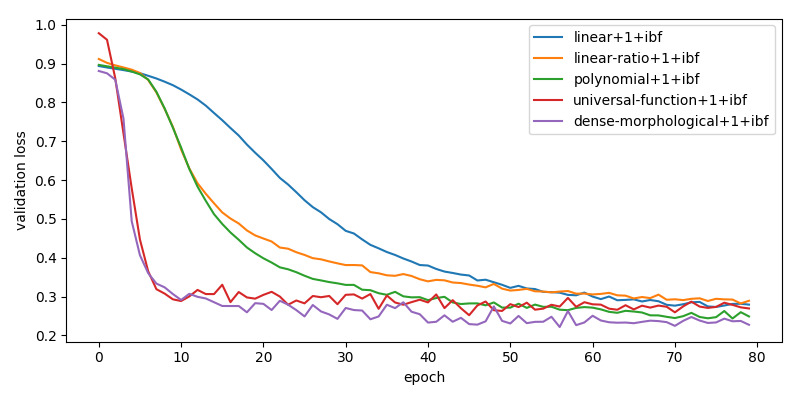
\includegraphics[width=\linewidth]{img/idx/model-convergence}
		\caption{first 80 epochs of loss of generic models with \textbf{ibf} in kernel size of 1.}
		\label{fig:all-loss}
	\end{figure}
	
	An important difference in the speed of convergence between models is observed.
	An analysis of this figure allows the aggregation of model types and speed: 
	
	\begin{itemize}
		\item Slow converging models: polynomials models converge slowly as well as the majority of linear or linear-ratio models.
		\item Fast converging models: universal-functions and dense-morphological are the fastest to converge (less than 30 iterations)
	\end{itemize}
	
	A subset of slow and fast converging models could be evaluated in term of sensitivity against initialization. It shows that the dense morphological followed by universal function {approximator convergence faster than the other. Regardless of the used module nor kernel size.}
	
	\newpage
	\subsubsection{Limits of Deepindices}
	Shadows can be a relatively hard problem to solve in image processing, the proposed models are able to correctly separate vegetation from soil even with shadowy images, as shown in Figure \ref{fig:correct-vi-soil-discrimination}. In addition, the  {Figure} \ref{fig:visual-comparison} in the  Appendix \ref{sec:appendices} shows the impacts of various acquisition factors, such as shadow, noise, specular or thin \mbox{vegetation features.}
	
	
	\begin{figure}[H]
		\centering
		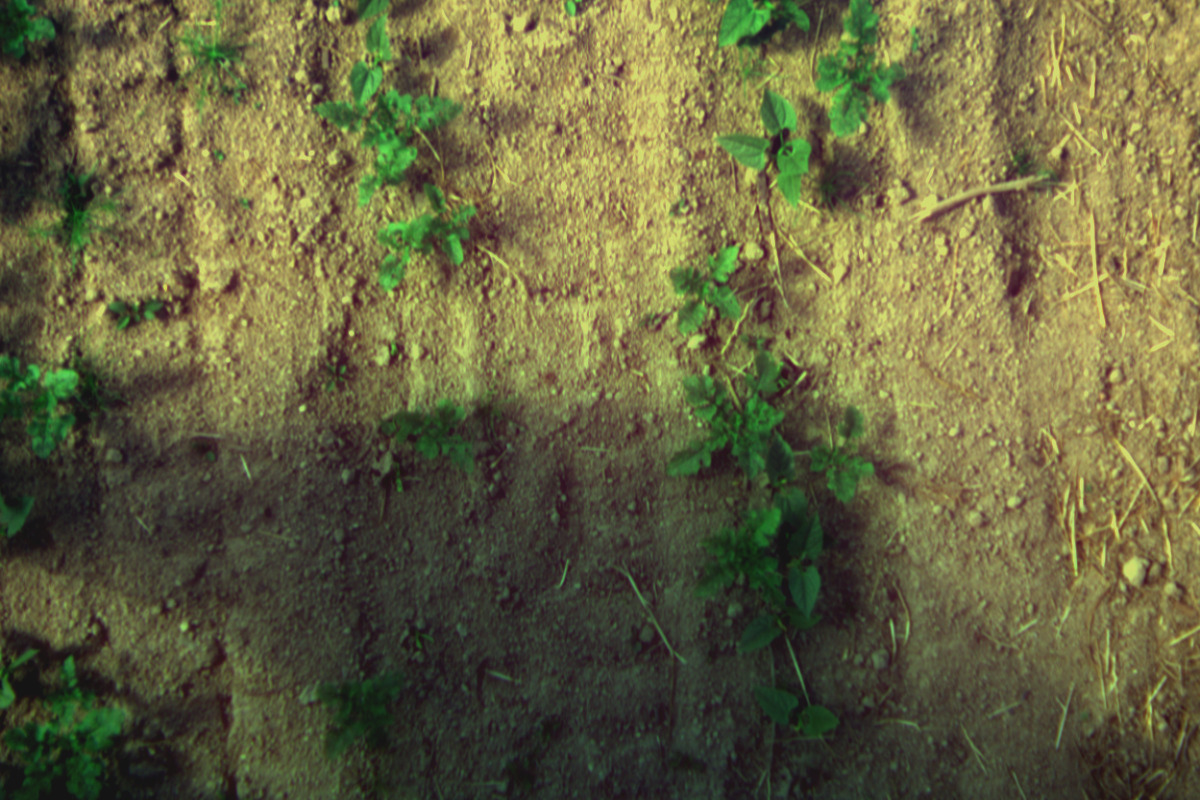
\includegraphics[width=0.45\linewidth]{img/idx/0090-false}
		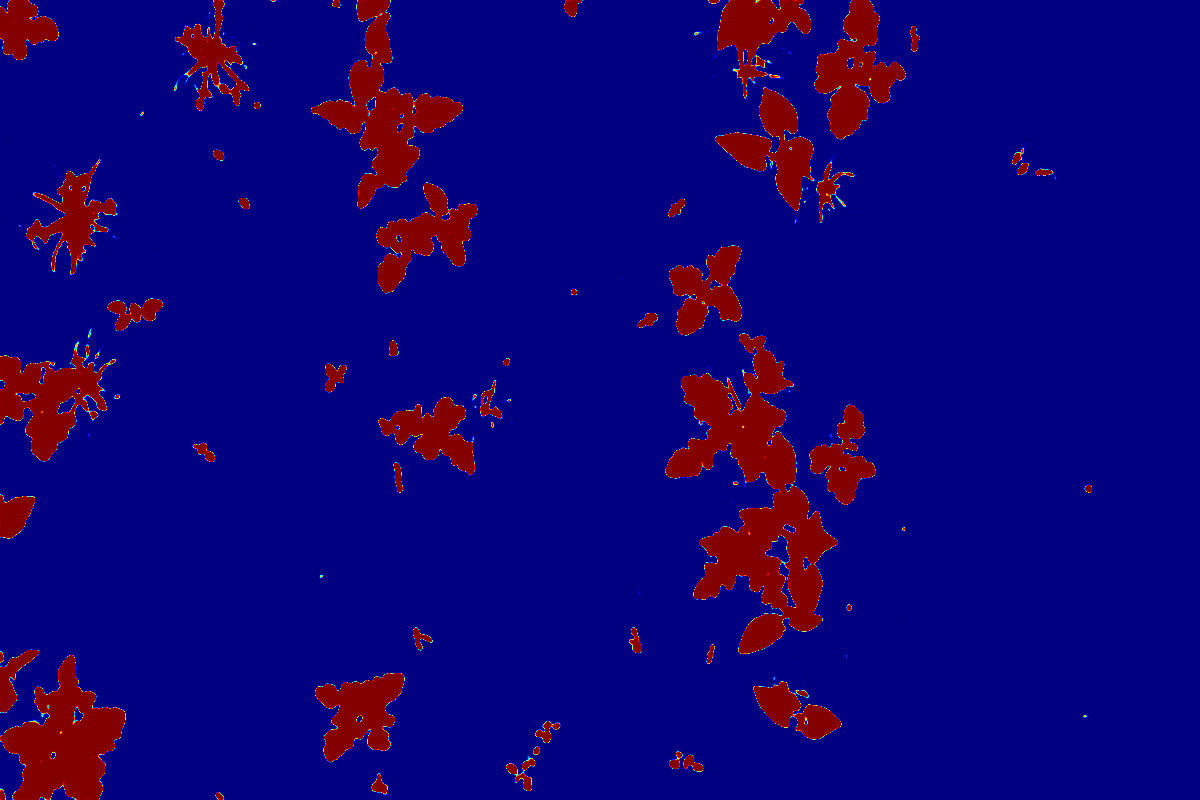
\includegraphics[width=0.45\linewidth]{img/idx/0090}
		\caption{Correct vegetation/soil discrimination despite shadows.}
		\label{fig:correct-vi-soil-discrimination}
	\end{figure}
	
	Some problem occurs when there are abrupt transitions between shadowed and light areas of an image as shown in Figure \ref{fig:bad-vi-soil-discrimination}.
	
	\begin{figure}[H]
		\centering
		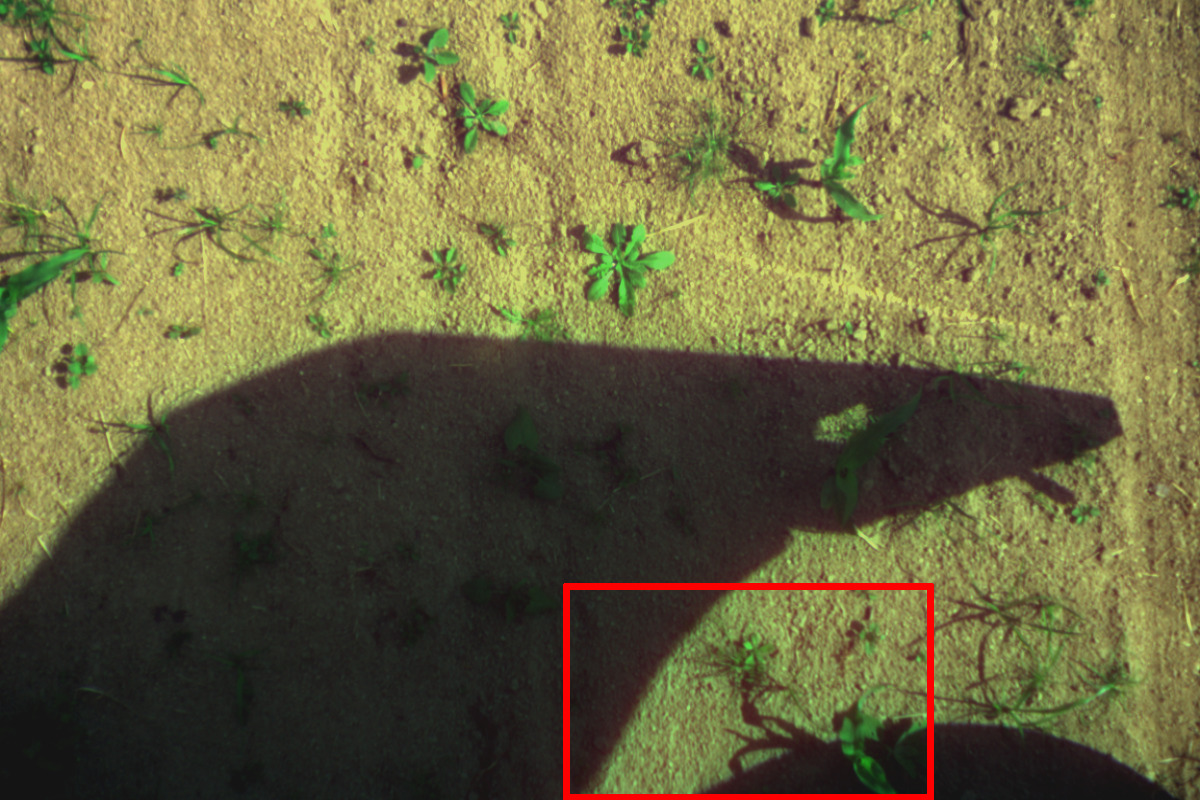
\includegraphics[width=0.45\linewidth]{img/idx/0400-false}
		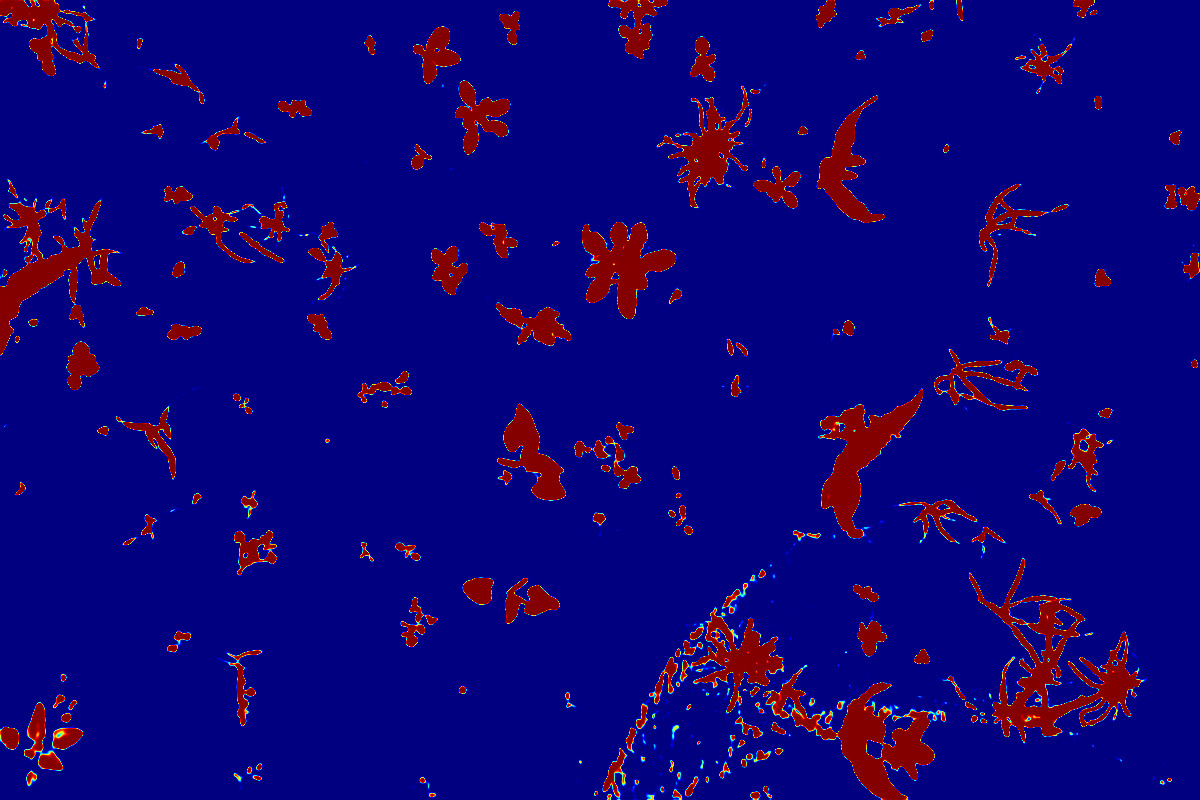
\includegraphics[width=0.45\linewidth]{img/idx/0400}
		\caption{Vegetation/soil discrimination issue with abrupt transition between shadow and light.}
		\label{fig:bad-vi-soil-discrimination}
	\end{figure}
	
	It appears that the discrimination error appears where the shadow is cast by a solid object, resulting in edge diffraction that creates small fringes on the soil and vegetation. A lack of such images in the training dataset could explain the model failure. Data augmentation could be used to obtain a training model containing such images, from cloud shadows to solid objects shadows. Further work is needed to estimate the benefit of such a data augmentation on the developed models.
	
	The smallest parts of the vegetation (less than 1 pixel, such as small monocotyledon leaves or plant stems) cannot be detected because of a strong spectral mixture. This limitation is due to the acquisition conditions (optics, CCD resolution and elevation) and should be considered as is. As vegetation with a width over 1 pixel is correctly segmented by our approach, the acquisition parameters should be chosen so that the smallest parts of vegetation that are required by an application are larger than 1 pixel in the resulting image.
	
	A few spots of specular light can also be observed on images, particularly on leaves. These spots are often unclassified (or classified as soil). This modifies the shape of the leaves by creating holes inside them. This problem can be seen on Figure \ref{fig:bad-specular}. Leaves with holes are visible on the left and the middle of the top bean row. It would be interesting to train the network to detect and assign them to a dedicated class. 
	
	\begin{figure}[H]
		\centering
		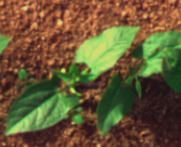
\includegraphics[width=0.3\linewidth]{img/idx/0020-false}
		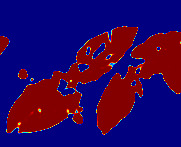
\includegraphics[width=0.3\linewidth]{img/idx/0020}
		\caption{Vegetation/soil discrimination issue caused by specular lights on leaves.}
		\label{fig:bad-specular}
	\end{figure}
	
	Next the location of the detected spots could be studied to re-assign them to two classes: specular-soil and specular-vegetation. To perform this step, a semantic segmentation could be set up to identify the surrounding objects of the holes specifically. It would be based on the UNet model, which performs a multi-scale approach by calculating, treating and re-convolving images of lower resolutions.
	
	More generally, the quality of the segmentation between soil and vegetation strongly influences the discrimination between crop and weed, which remains a major application following this segmentation task. Three categories of troubles have been identified: the plants size, the ambient light variations (shades, specular light spots), and the morphological complexity of the studied objects.
	
	The size of the plants mainly impacts their visibility on the acquired images. It is not obviously related to the ability of the algorithm to classify them. However, it leads to the absence of essential elements such as monocotyledon weeds at an early vegetation stage. A solution is proposed by setting the acquisition conditions to let the smallest vegetation part be over \mbox{1 pixel.}
	
	Conversely, the variations of ambient light should be treated by the classification algorithm. As previously mentioned, shadow management needs an improvement of the learning base, and specular light spots could be treated by a multi-scale approach. Their influence on the discrimination step should be major. Indeed, they influence the shape of the objects classified as plants, which is a useful criterion to discriminate crops from weeds. 
	The morphological complexity of the plants can be illustrated by the presence of stems. In our case, bean stems are similar to weed leaves. This problem should be treated by the discrimination step. The creation of a stem class (in addition to the weed and crop classes) will be studied in particular.
	
	\newpage
	\section{Conclusions}
	\label{sec:conclusions}
	
	In this work, different standard vegetation indices have been evaluated as well as different methods to estimate new DeepIndices through different types of equations that can reconstruct the others. Among the 89 standard vegetation indices tested, the MTVI (Modified Triangular Vegetation Index 1) gives the best vegetation segmentation. Standard indices remain sub-optimal even if they are downstream optimized with a linear regression because they are usually used on calibrated reflectance data. The results allow us to conclude that any simple linear combination is just more efficient ($+4.87\%$ mIoU) than any standard indices by taking into account all spectral bands and few transformations. The results also suggest that un-calibrated data can be used in proximal sensing applications for both standard indices and DeepIndices with good performances.
	
	We therefore agree that it is important to optimize both the arithmetic structure of the equation and the coefficients of the spectral bands, that is why our automatically generated indices are much more accurate. The best model is much more efficient by $+8.48\%$ compared to the best standard indices and by $+18.21\%$ compared to NDVI. Also the two modules \textbf{ibf}, \textbf{sprb} and the initial image transformation show a significant improvement. The developed DeepIndices allow to take into account the lighting variation within the equation. It makes possible to abstract from a difficult problem which is the data calibration. Thus, partially shaded images are correctly evaluated, which is not possible with standard indices since they use sprectum measurement that change with shades. However, it would be interesting to evaluate the performance of standard indices and DeepIndices on calibrated reflectance data.
	
	These results suggest that deep learning algorithms are a useful tool to discover the spectral band combinations that identify the vegetation in multi spectral camera. Another conclusion from this research is about the genericity of the methodology developed. This study presents a first experiment employed in field images with the objective of finding deep vegetation indices and demonstrates their effectiveness compared to standard vegetation indices. This paper's contribution improves the classical methods of vegetation index development and allows the generation of more precise indices (i.e., DeepIndices). The same kind of conclusion may arise from this methodology applied on remote sensing indices to discriminates other surfaces (roads, water, snow, shadows, etc).

	\newpage
	\paragraph*{Author Contributions}{
		Conceptualization, Vayssade, J.-A.;
		data curation, Vayssade, J.-A.;
		formal analysis, Vayssade, J.-A.;
		funding acquisition, Jones, G and Paoli, J.-N.;
		investigation, Vayssade, J.-A.;
		methodology, Vayssade, J.-A.; 
		project administration, Paoli.J-N. and Jones, G;
		resources, Paoli.J-N. and Jones, G;
		software, Vayssade, J.-A.;
		supervision, Paoli, J.-N. and Jones, G;
		validation, Paoli, J.-N.; Gée, C. and Jones, G.;
		visualization, Vayssade, J.-A.;
		writing---original draft preparation, Vayssade, J.-A.;
		writing---review and editing, Vayssade, J.-A.; Paoli, J.-N.; Gée, C. and Jones, G.;
		All authors have read and agreed to the published version of the manuscript.
	}

	\paragraph*{Funding}{This project is funded by ANR Challenge RoSE and the Horizon 2020 project IWMPRAISE.}

	\paragraph*{Data Availability}{Data in this study is publicly available at \url{https://data.inrae.fr/dataset.xhtml?persistentId=doi:10.15454/DSQC8N}, using Creative Common CC0 1.0 Public Domain Dedication licence}

	\paragraph*{Acknowledgments}{We would like to thank Masson Jean-Benoit for the realization of the metal gantry which allowed us to position the camera at different heights, it was used in particular for the calibration of the camera and the band registration. We also thank Djemai Mehdi for the spelling correction of the English. And we thank Aubry Clément and Cozic Thibault of the company SITIA for their help in interfacing the camera with the used robot ``Trecktor''.}

	\paragraph*{Conflicts Of Interest}{The authors declare no conflict of interest. The funders had no role in the design of the study; in the collection, analyses, or interpretation of data; in the writing of the manuscript, or in the decision to publish the results.}

	\section*{Appendices and supplementary material}
	\label{sec:appendices}
	
	\begin{table}[H]
		\centering
		$b = \rho_{0}, g = \rho_{1}, r = \rho_{2}, e = \rho_{3}, u = \rho_{4}, n = \rho_{5}$ \\
        \rowcolors{0}{gray!10}{white}
		\begin{tabular}{|l|l|}
			\hline \textbf{Model}  &	\textbf{Equation} \\ \hline
			
			Modified Triangular Vegetation Index 1                 & {$1.2*(1.2*(n-g)-2.5*(r-g))$} \\
			Modified Chlorophyll Absorption In Reflectance Index 1 & {$1.2*(2.5*(n-r)-1.3*(n-g))$} \\
			Enhanced Vegetation Index 2                            & {$2.4*(n-r) / (n+r+1)$} \\
			Soil Adjusted Vegetation Index                         & {$1.5*(n-r, n+r+0.5)$} \\
			Soil And Atmospherically Resistant VI 3  			   & {$1.5*(n-r, n+r)$} \\
			Enhanced Vegetation Index 3                            & {$2.5*(n-r) / (n+2.4*r+1)$} \\
			Global Environment Monitoring Index                    & {$\frac{2*(n^2 -r^2)+1.5*n+0.5*r}{n+r+0.5} * (1-n/4) - \frac{r-0.125}{1+r}$} \\
			Adjusted Transformed Soil Adjusted VI                  & {$a*\frac{n-a*r-0.03}{a*n+r-a*0.03+0.08*(1+a)**2}$ $a=1.22$} \\
			NDVI                                                   & {$(n-r) / (n+r)$} \\ \hline
		\end{tabular}
		\caption{Top optimized fixed vegetation model equations}
		\label{tab:fixed-veg-indices-eqn}
	\end{table}
	
    \newpage
    \null
    \vfill
	\begin{figure}[H]
		\centering
		\UnframedBox{.5cm}{.5cm}{$ $} \hspace{-1em}
		\FramedBox{.5cm}{0.2\linewidth}{Noise} \hspace{-1em}
		\FramedBox{.5cm}{0.2\linewidth}{Shadow} \hspace{-1em}
		\FramedBox{.5cm}{0.2\linewidth}{Thin} \hspace{-1em}
		\FramedBox{.5cm}{0.2\linewidth}{Specular} \hspace{-1em}
		
		\FramedBox{0.2\linewidth}{.5cm}{\rotatebox{90}{RGB}} \hspace{-1em}
		%\FramedBox{0.2\linewidth}{0.2\linewidth}{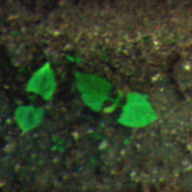
\includegraphics[width=0.2\linewidth]{img/idx/small-illustration/noise1/rgb}}
		\FramedBox{0.2\linewidth}{0.2\linewidth}{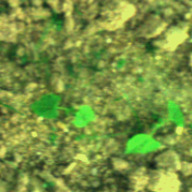
\includegraphics[width=\linewidth]{img/idx/small-illustration/noise3/rgb}} \hspace{-1em}
		\FramedBox{0.2\linewidth}{0.2\linewidth}{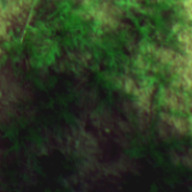
\includegraphics[width=\linewidth]{img/idx/small-illustration/shadow4/rgb}} \hspace{-1em}
		\FramedBox{0.2\linewidth}{0.2\linewidth}{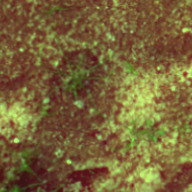
\includegraphics[width=\linewidth]{img/idx/small-illustration/small1/rgb}} \hspace{-1em}
		\FramedBox{0.2\linewidth}{0.2\linewidth}{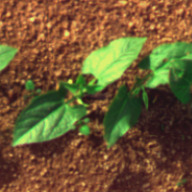
\includegraphics[width=\linewidth]{img/idx/small-illustration/spec1/rgb}} \hspace{-1em}
		
		\FramedBox{0.2\linewidth}{.5cm}{\rotatebox{90}{Ground Truth}} \hspace{-1em}
		%\FramedBox{0.2\linewidth}{0.2\linewidth}{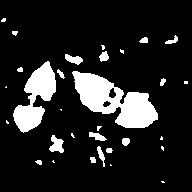
\includegraphics[width=\linewidth]{img/idx/small-illustration/noise1/gt}}
		\FramedBox{0.2\linewidth}{0.2\linewidth}{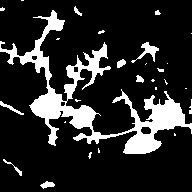
\includegraphics[width=\linewidth]{img/idx/small-illustration/noise3/gt}} \hspace{-1em}
		\FramedBox{0.2\linewidth}{0.2\linewidth}{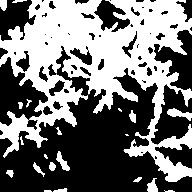
\includegraphics[width=\linewidth]{img/idx/small-illustration/shadow4/gt}} \hspace{-1em}
		\FramedBox{0.2\linewidth}{0.2\linewidth}{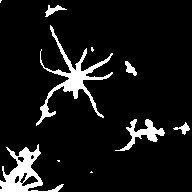
\includegraphics[width=\linewidth]{img/idx/small-illustration/small1/gt}} \hspace{-1em}
		\FramedBox{0.2\linewidth}{0.2\linewidth}{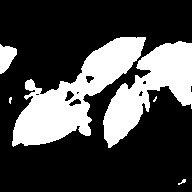
\includegraphics[width=\linewidth]{img/idx/small-illustration/spec1/gt}} \hspace{-1em}
		
		\FramedBox{0.2\linewidth}{.5cm}{\rotatebox{90}{dense 7 ibf+sprb}} \hspace{-1em}
		%\FramedBox{0.2\linewidth}{0.2\linewidth}{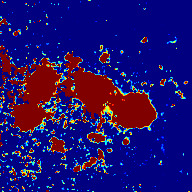
\includegraphics[width=\linewidth]{img/idx/small-illustration/noise1/dense-7-ibf-sprb}}
		\FramedBox{0.2\linewidth}{0.2\linewidth}{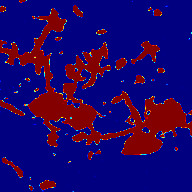
\includegraphics[width=\linewidth]{img/idx/small-illustration/noise3/dense-7-ibf-sprb}} \hspace{-1em}
		\FramedBox{0.2\linewidth}{0.2\linewidth}{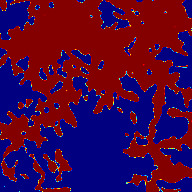
\includegraphics[width=\linewidth]{img/idx/small-illustration/shadow4/dense-7-ibf-sprb}} \hspace{-1em}
		\FramedBox{0.2\linewidth}{0.2\linewidth}{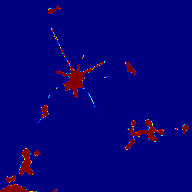
\includegraphics[width=\linewidth]{img/idx/small-illustration/small1/dense-7-ibf-sprb}} \hspace{-1em}
		\FramedBox{0.2\linewidth}{0.2\linewidth}{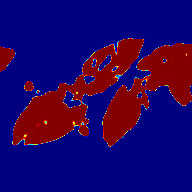
\includegraphics[width=\linewidth]{img/idx/small-illustration/spec1/dense-7-ibf-sprb}} \hspace{-1em}
		
		\FramedBox{0.2\linewidth}{.5cm}{\rotatebox{90}{linear 1 baseline}} \hspace{-1em}
		%\FramedBox{0.2\linewidth}{0.2\linewidth}{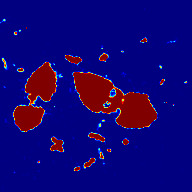
\includegraphics[width=\linewidth]{img/idx/small-illustration/noise1/linear-1-baseline}}
		\FramedBox{0.2\linewidth}{0.2\linewidth}{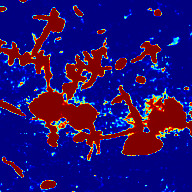
\includegraphics[width=\linewidth]{img/idx/small-illustration/noise3/linear-1-baseline}} \hspace{-1em}
		\FramedBox{0.2\linewidth}{0.2\linewidth}{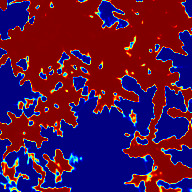
\includegraphics[width=\linewidth]{img/idx/small-illustration/shadow4/linear-1-baseline}} \hspace{-1em}
		\FramedBox{0.2\linewidth}{0.2\linewidth}{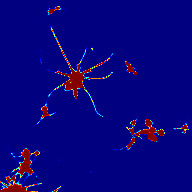
\includegraphics[width=\linewidth]{img/idx/small-illustration/small1/linear-1-baseline}} \hspace{-1em}
		\FramedBox{0.2\linewidth}{0.2\linewidth}{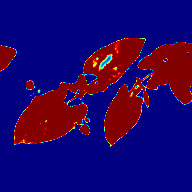
\includegraphics[width=\linewidth]{img/idx/small-illustration/spec1/linear-1-baseline}} \hspace{-1em}
		
		\FramedBox{0.2\linewidth}{.5cm}{\rotatebox{90}{MTVI1}} \hspace{-1em}
		%\FramedBox{0.2\linewidth}{0.2\linewidth}{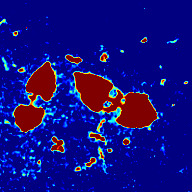
\includegraphics[width=\linewidth]{img/idx/small-illustration/noise1/modifed}}
		\FramedBox{0.2\linewidth}{0.2\linewidth}{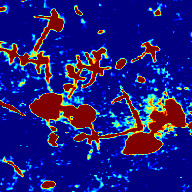
\includegraphics[width=\linewidth]{img/idx/small-illustration/noise3/modifed}} \hspace{-1em}
		\FramedBox{0.2\linewidth}{0.2\linewidth}{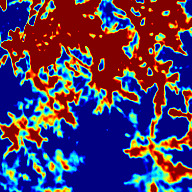
\includegraphics[width=\linewidth]{img/idx/small-illustration/shadow4/modifed}} \hspace{-1em}
		\FramedBox{0.2\linewidth}{0.2\linewidth}{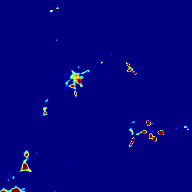
\includegraphics[width=\linewidth]{img/idx/small-illustration/small1/modifed}} \hspace{-1em}
		\FramedBox{0.2\linewidth}{0.2\linewidth}{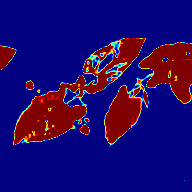
\includegraphics[width=\linewidth]{img/idx/small-illustration/spec1/modifed}} \hspace{-1em}
		
		\FramedBox{0.2\linewidth}{.5cm}{\rotatebox{90}{NDVI}} \hspace{-1em}
		%\FramedBox{0.2\linewidth}{0.2\linewidth}{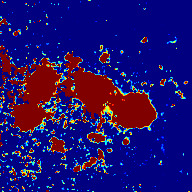
\includegraphics[width=\linewidth]{img/idx/small-illustration/noise1/ndvi}}
		\FramedBox{0.2\linewidth}{0.2\linewidth}{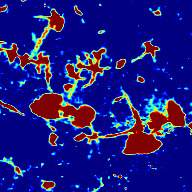
\includegraphics[width=\linewidth]{img/idx/small-illustration/noise3/ndvi}} \hspace{-1em}
		\FramedBox{0.2\linewidth}{0.2\linewidth}{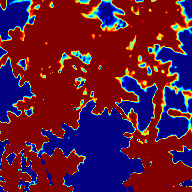
\includegraphics[width=\linewidth]{img/idx/small-illustration/shadow4/ndvi}} \hspace{-1em}
		\FramedBox{0.2\linewidth}{0.2\linewidth}{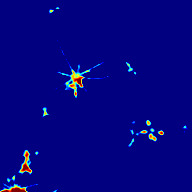
\includegraphics[width=\linewidth]{img/idx/small-illustration/small1/ndvi}} \hspace{-1em}
		\FramedBox{0.2\linewidth}{0.2\linewidth}{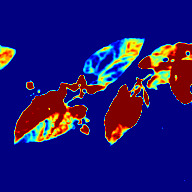
\includegraphics[width=\linewidth]{img/idx/small-illustration/spec1/ndvi}} \hspace{-1em}
	
		\caption{Visual comparison between some relevant models. NDVI (63.98 mIoU), MTVI1 (73.71 mIoU), linear 1 baseline (78.58 mIoU), dense 7 ibf-sprb (82.19 mIoU). 
		Blue indicates sure soil, red indicates sure vegetation, and the other colors indicate uncertainty.}
	\label{fig:visual-comparison}
	\end{figure}
    \vfill

	%\begin{specialtable}[H]
	%	\centering
	%	$b = \rho_{0}, g = \rho_{1}, r = \rho_{2}, e = \rho_{3}, u = \rho_{4}, n = \rho_{5}$ \\
	%	\begin{tabularx}{\linewidth} {|l|X|}
	%		 ine \textbf{model}  &	\textbf{equation} \\  ine
	%		 ine Tasselled Cap Soil Brightness Index MSS 	& $-0.283*g-0.660*r+0.577*u+0.388*n$ \\
	%		 ine Misra Green Vegetation Index 			& $-0.386*g-0.53*r+0.535*u+0.532*n$ \\
	%		 ine Enhanced Vegetation Index 2 				& $2.4 (n-r) \div (n+r+1)$ \\
	%		 ine Modified Soil Adjusted Vegetation Index 	& $(2*n+1-\sqrt{(2*n+1)^2-8*(n-r)}) \div 2$ \\
	%		 ine Enhanced Vegetation Index 3 				& $2.5 (n-r) \div (n+2.4*r+1)$ \\
	%		 ine Soil And Atmospherically Resistant Vegetation Index 3 & $1.5(n-r)\div(n+r+0.5)$ \\
	%		 ine Soil Adjusted Vegetation Index 				& $1.5(n-r) \div (n+r+0.5)$ \\
	%		 ine Adjusted Transformed Soil Adjusted VI 		& { $\frac{a(n-a*r-b)}{a*n+r-a*b+X*(1+a)**2}$\\ $X,a,b=[0.08, 1.22, 0.03]$} \\
	%		 ine Triangular Vegetation Index 					& $1.2*(1.2*(n-g)-2.5*(r-g))$ \\
	%		 ine Soil And Atmospherically Resistant Vegetation Index & {$\frac{(1+L) (n-(r*R-y*(r*b-r*R)))}{n+(R*r-y*(r*b-r*R))+L}$ \\ $L=0.5, R = 1, y = 1$} \\
	%		 ine Modified Triangular Vegetation Index 1 				  & $1.2*(1.2*(n-g)-2.5*(r-g))$ \\
	%		 ine Modified Chlorophyll Absorption In Reflectance Index 1 & $1.2*(2.5*(n-r)-1.3*(n-g))$ \\
	%		 ine Global Environment Monitoring Index 					  & $2((n^2-r^2) + 1.5n + 0.5r)(1-0.25*n) \div (n + r + 0.5) - (r-0.125)\div(1-r)$ \\
	%		 ine Spectral Polygon Vegetation Index 					  & $0.4(3.7(n-r)) - 1.2|g-r|$ \\
	%		 ine Ashburn Vegetation Index 							  & $2*n - r$ \\
	%		 ine NDVI 												  & $(n-r) \div (n+r)$ \\
	%		 ine
	%	\end{tabularx}
	%	\vspace{-1em}
	%	\caption{Top optimized fixed vegetation model equations}
	%	\label{tab:fixed-veg-indices-eqn}
	%\end{table}
	
	%	\colorbox{orange}{A supprimer ?}
	%	
	%	\begin{specialtable}[H]
	%		\centering
	%		%$b = \rho_{450}, g = \rho_{570}, r = \rho_{650}, e = \rho_{710}, u = \rho_{730}, n = \rho_{850}$ \\
	%		$b = \rho_{0}, g = \rho_{1}, r = \rho_{2}, e = \rho_{3}, u = \rho_{4}, n = \rho_{5}$ \\
	%		
	%		\begin{tabularx}{\textwidth}{ |l|X| }
	%			 ine
	%			\textbf{Model} & \textbf{equation} \\
	%			 ine Adventiced Transformed Soil Adjusted VI  & $a(n-a*r-b) \div (a*n+r-a*b+X*(1+a)**2)$ \newline $X,a,b=[0.08, 1.22, 0.03]$ \\
	%			 ine Anthocyanin Refectance Index & ${1}\div{b} - {1}\div{e}$ \\
	%			 ine Ashburn Vegetation Index & $2*n - r$ \\
	%			 ine Atmospherically Resistant Vegetation Index & $(n-r-y*(r-b)) \div (n+r-y*(r-b))$ \newline $y=0.5$ \\
	%			 ine Atmospherically Resistant Vegetation Index 2 & $(y*(n-r)) \div (n+r)$ \newline $x,y=-0.18, 1.17$ \\
	%			 ine Average Reflectance 750 to 850 & $(e+u+n) \div 3$ \\
	%			 ine Blue Wide Dynamic Range Vegetation Index & $(2n-b) \div (2n+b)$ \\
	%			 ine Browning Reflectance Index & $(1\div b - 1 \div e) \div n$ \\
	%			 ine CRI 700 & $g^{-1} - e^{-1}$ \\
	%			 ine Canopy Chlorophyll Content Index & $((n-u)\div(n+u)) \div ((n-r)\div(n+r))$ \\
	%			 ine Chlorophyll Absorption Ratio Index & $(e \div r) \sqrt{(a*r +r + (g-(e-g)/150*g))^2} \div \sqrt{a^2}$ \newline $a = (e-g)/150$ \\
	%			 ine Chlorophyll Absorption Ratio Index 2 & $(e \div r) |a*r+r+g-a*g| \div \sqrt{a^2}$ \newline $a = (e-g)/150$ \\
	%			 ine Chlorophyll Green & $(u \div g)^{-1}$ \\
	%			 ine Chlorophyll Index Green & $(n \div g)^{-1}$ \\
	%			 ine Chlorophyll Index RedEdge & $n \div u -1$ \\
	%			 ine Chlorophyll Index RedEdge 710 & $u \div e -1$ \\
	%			 ine Chlorophyll RedEdge & $(n \div u)^{-1}$ \\
	%			 ine Chlorophyll Vegetation Index & $n*(r-g^2)$ \\
	%			 ine Coloration Index & $(r-b) \div r$ \\
	%			 ine Corrected Transformed Vegetation Index & $ndvi/|ndvi| * tf.sqrt(ndvi)$ \\
	%			 ine Datt 1 & $(n-e) \div (n-r)$ \\
	%			 ine Datt 4 & $r \div (g*e+1)$ \\
	%			 ine Datt 6 & $n \div (g*e)$ \\
	%			 ine Difference NIR Green Vegetation Index & $n-g$ \\
	%			 ine Differenced Vegetation Index MSS & $2.4*n - (e+u) \div 2$ \\
	%			 ine Double Difference Index & $(u-e) - (e-r)$ \\
	%			 ine Enhanced Vegetation Index & $2.5(n-r)\div(n+6*r-7.5*b+1)$ \\
	%			 ine
	%		\end{tabularx}
	%	\end{table}
	%	
	%	\begin{specialtable}[H]
	%		\begin{tabularx}{\textwidth}{ |l|X| }
	%			 ine
	%			\textbf{Model} & \textbf{equation} \\  ine
	%			 ine Enhanced Vegetation Index 2 & $2.4 (n-r) \div (n+r+1)$ \\
	%			 ine Enhanced Vegetation Index 3 & $2.5 (n-r) \div (n+2.4*r+1)$ \\
	%			 ine Gitelson 2 & $(u-n)\div(r-u) -1$ \\
	%			 ine Global Environment Monitoring Index & $2((n^2-r^2) + 1.5n + 0.5r)(1-0.25*n) \div (n + r + 0.5) - (r-0.125)\div(1-r)$ \\
	%			 ine Global Vegetation Moisture Index & $((n+0.1) - (e+0.02))\div((n+0.1) + (e+0.02))$ \\
	%			 ine Green Atmospherically Resistant Vegetation Index & $(n-(g-(b-r)))\div(n-(g+(b-r)))$ \\
	%			 ine Green Blue NDVI & $(n-g-b)\div(n+g+b)$ \\
	%			 ine Green Leaf Index & $(2*g-r-b)\div(2*g+r+b)$ \\
	%			 ine Green Normalized Difference Vegetation Index & $(n-g)\div(n+g)$ \\
	%			 ine Green Optimized Soil Adjusted Vegetation Index & $(n-g)\div (n+2g)$ \\
	%			 ine Green Red NDVI & $(n-g-r)\div(n+g+r)$ \\
	%			 ine Green Soil Adjusted Vegetation Index & $(n-g) (1+L) \div (n+g+L) $ \newline $L=1$ \\
	%			 ine Ideal Vegetation Index & $(n-B)\div(A*r)$ \newline $A=1, B=1$ \\
	%			 ine Infrared Percentage Vegetation Index & $(n \div 2(n+r))*(ndvi+1)$ \\
	%			 ine Intensity & $(r+g+b) \div 3.5 $ \\
	%			 ine MCARI\_OSAVI & $((e-r) - 0.2*(e-g)(e \div r)) \div (1.16(n-r)\div (n+r+0.16))$ \\
	%			 ine MCARI\_OSAVI750 & $((u-e) - 0.2*(u-g)(u \div e)) \div (1.16(n-e)\div(n+r+0.16))$ \\
	%			 ine Misra Green Vegetation Index & $-0.386*g-0.53*r+0.535*u+0.532*n$ \\
	%			 ine Misra Non Such Index & $0.404*g-0.039*r+0.505*u+0.762*n$ \\
	%			 ine Misra Soil Brightness Index & $0.406*g+0.6*r+0.645*u+0.243*n$ \\
	%			 ine Misra Yellow Vegetation Index & $0.723*g-0.597*r+0.206*u-0.278*n$ \\
	%			 ine Modified Anthocyanin Reflectance Index & $(g^{-1} - e^{-1})n$ \\
	%			 ine Modified Chlorophyll Absorption In Reflectance Index & $(((e-r)-0.2*(e-g))*e) \div r$ \\
	%			 ine Modified Chlorophyll Absorption In Reflectance Index 1 & $1.2*(2.5*(n-r)-1.3*(n-g))$ \\
	%			 ine Modified Simple Ratio & $(n-b)\div(r-b)$ \\
	%			 ine Modified Simple Ratio 670 800 & $(n \div r -1) \div \sqrt{n \div r +1}$ \\
	%			 ine Modified Simple Ratio 705 750 & $(u \div e -1) \div \sqrt{u \div e +1}$ \\
	%			 ine Modified Soil Adjusted Vegetation Index & $(2*n+1-\sqrt{(2*n+1)^2-8*(n-r)}) \div 2$ \\
	%			 ine
	%		\end{tabularx}
	%	\end{table}
	%	
	%	\begin{specialtable}[H]
	%		\begin{tabularx}{\textwidth}{ |l|X| }
	%			 ine
	%			\textbf{Model} & \textbf{equation} \\  ine
	%			 ine Modified Triangular Vegetation Index 1 & $1.2*(1.2*(n-g)-2.5*(r-g))$ \\
	%			 ine NDVI & $(n-r) \div (n+r)$ \\
	%			 ine Norm G & $g \div (n+r+g)$ \\
	%			 ine Norm Nir & $n \div(n+r+g)$ \\
	%			 ine Norm R & $r \div (n+r+g)$ \\
	%			 ine Pan NDVI & $(n-g-r-b) \div (n+g+r)$ \\
	%			 ine Red Blue NDVI & $(n-r-b) \div (n+r+b)$ \\
	%			 ine RedEdge Inflection Point & $700+40((r+n)/2-e)\div (u-e)$ \\
	%			 ine RedEdge Position Linear Interpolation & $700+40((r+n)/2-e) \div (u-e)$ \\
	%			 ine Shape Index & $(2*r-g-b)\div (g-b)$ \\
	%			 ine Soil Adjusted Vegetation Index & $1.5(n-r, n+r+0.5)$ \\
	%			 ine Soil And Atmospherically Resistant Vegetation Index & $(1+L) (n-(r*R-y*(r*b-r*R))) \div (n+(R*r-y*(r*b-r*R))+L)$ \newline $L=0.5, R = 1, y = 1$ \\
	%			 ine Soil And Atmospherically Resistant Vegetation Index 2 & $2.5(n-r) \div (1+n+6*r-7.5*b)$ \\
	%			 ine Soil And Atmospherically Resistant Vegetation Index 3 & $1.5(n-r)\div(n+r+0.5)$ \\
	%			 ine Specific Leaf Area Vegetation Index & $n \div (r+u)$ \\
	%			 ine Spectral Polygon Vegetation Index & $0.4(3.7(n-r)) - 1.2|g-r|$ \\
	%			 ine Structure Intensive Pigment Index 1 & $(n-b) \div (n-r)$ \\
	%			 ine Structure Intensive Pigment Index 2 & $(n-g) \div (n-r)$ \\
	%			 ine TCARI\_OSAVI & $(3*(e-r) - 0.2*(e-g)(e \div r)) \div ((1.16*(n-r))\div(n+r+0.16))$ \\
	%			 ine Tasselled Cap Non Such Index MSS & $-0.016*g+0.131*r-0.425*u+0.882*n$ \\
	%			 ine Tasselled Cap Soil Brightness Index MSS & $-0.283*g-0.660*r+0.577*u+0.388*n$ \\
	%			 ine Tasselled Cap Yellow Vegetation Index MSS & $-0.899*g-0.428*r+0.076*u+0.041*n$ \\
	%			 ine Transformed Chlorophyll Absorption Ratio & $3((e-r)-0.2(e-g)(e \div r))$ \\
	%			 ine Transformed Chlorophyll Absorption Ratio 2 & $3((u-e)-0.2*(u-g)*(u \div e))$ \\
	%			 ine Transformed NDVI & $\sqrt{(n-r)\div(n+r)+0.5}$ \\
	%			 ine Triangular Chlorophyll Index & $1.2(e-g) - 1.5(r-g)*tf.sqrt{e \div r}$ \\
	%			 ine Triangular Vegetation Index & $-0.5 * (120*(u-g) - 200*(r-g))$ \\
	%			 ine Vegetation Condition Index & $(NDVI - \min_{NDVI}) \div (\max_{NDVI} - \min_{NDVI})$ \\
	%			 ine Vegetation Index 700 & $(e-r)\div(e+r)$ \\
	%			 ine Visible Atmospherically Resistant Index Green & $(g-r)\div(g+e-b)$ \\
	%			 ine
	%		\end{tabularx}
	%	\end{table}
	%	
	%	\begin{specialtable}[H]
	%		\begin{tabularx}{\textwidth}{ |l|X| }
	%			 ine
	%			\textbf{Model} & \textbf{equation} \\  ine
	%			 ine Visible Atmospherically Resistant Indices 700 & $(e-1.7*r+0.7*b) \div (e+2.3*r-1.3*b)$ \\
	%			 ine Wide Dynamic Range Vegetation Index & $(0.1*n-r) \div (0.1*n+r)$ \\
	%			 ine mCRIRE & $(g^{-1} - e^{-1})*n$ \\
	%			 ine mSR2 & $(u \div e) - (1 \div \sqrt{u \div e +1})$ \\
	%			 ine
	%		\end{tabularx}
	%		\caption{list of fixed vegetation models}
	%		\label{tab:fixed-veg-indices-models}
	%	\end{table}
	

	\newpage
	\section{Conclusion de chapitre}
	
	Dans cet article, de nouveaux indices de végétation (Deep Indices) ont été proposés. En partant de la définition d'une large quantité d'équations d'indices de végétation (89), il a été possible de déterminer deux équations simples qui généralisent la majorité d'entre elles, tout en considérant l'ensemble des bandes spectrales. Pour aller plus loin, des méthodes reposants sur des approximateurs de fonctions (développements de Taylor, polynômes de Bernstein, et opérateurs morphologiques) ont également été testées, de même que l'ajout de transformations des données d'entrée (déviation standard, matrice hessienne, \dots) ou de traitement du signal en amont des fonctions à optimiser (filtre passe-bas, passe-haut et passe-bande).
    
    Ces indices ont été développés au travers d'un outil d'apprentissage profond permettant des temps de traitement minimes. De plus, une fonction de perte adaptée permet d'optimiser ces indices pour obtenir la segmentation la plus proche de celle souhaitée. Un ensemble conséquent de 89 indices standards a également été optimisé en suivant cette démarche. Cela permet de comparer indices standards et indices proposés avec des degrés d'optimisations similaires.
    
    Ces indices ont été appris sur un ensemble de 91 images non calibrées et contenant des variations importantes des conditions d'acquisition. La taille du jeu d'apprentissage ne nécessite pas d'être plus conséquente, en revanche le choix des images et la représentation des différentes conditions d'acquisition dans des proportions spécifiques jouent un rôle important. Pour ce type de démarche, il est nécessaire de sous-représenter les images simples, acquises dans de bonnes conditions. L'utilisation de techniques d'augmentation de données (bruit de Perlin) renforce également la robustesse des indices appris. %Plus largement, ceci est un problème d'apprentissage lié au déséquilibre des classes (sol/végétation). \color{red} Je ne mettrais pas ncette dernière phrase qui pour moi en dit trop oun pas assez...\color{black}
    
    Les résultats montrent que certains indices standards peuvent proposer des résultats intéressants en termes de segmentation sol/végétation après optimisation. Le MTVI (Modified Triangular Vegetation Index 1) donne ainsi les meilleurs résultats ($\SI{73.71}{mIoU}$). A contrario, le NDVI, l'indice le plus utilisé dans la littérature, montre des résultats moyens ($\SI{63.98}{mIoU}$) pour cette tâche. Ces indices standards, sont facilement dépassés par une simple régression linéaire ($\SI{78.58}{mIoU}$). Et ils sont largement moins performants que les indices proposés dans notre étude ($\SI{82.19}{mIoU}$). % Ces derniers reposent sur des approximateurs de fonction et incluant un traitement du signal.
    Certains artefacts ne sont toutefois pas traités par les Deep-Indices. C'est le cas de la réflexion spéculaire (figure \ref{fig:bad-specular}), des aberrations chromatiques visibles en bordure d'ombre (figure \ref{fig:bad-vi-soil-discrimination}) et des pixels présentant un mélange spectral (figure \ref{fig:visual-comparison}), souvent en bordure de feuille, ou sur les feuilles fines.
    
    %Dans le chapitre précédent, nous avons défini avec succès les indices de végétation les plus performants et robuste aux changements d'illumination globaux (environnement) et locaux (ombres, bruit). À notre connaissance, il n'existe pas d'études comparables. Ces indices optimisés représentent donc une avancée considérable en télédétection et en proxi-détection. En particulier la où l'utilisation d'une calibration radiométrique n'est pas envisageable. Ces indices optimisés représentent la première étape de la phase de segmentation.
    
    Grâce à ces nouveaux indices, ne nécessitant pas de calibration, nous avons répondu efficacement à la première question de l'étape de segmentation : comment discriminer la végétation du reste de la scène ? Ceci constitue un des apports scientifiques de cette thèse. Maintenant que la première étape de segmentation est achevée, la seconde question est : comment différencier les individus au sein d'un couvert végétal ? Pour cela, plusieurs échelles sont possibles : composantes connexes, plantes, pixels, \dots. Les méthodes utilisables dépendent de ce choix et le chapitre suivant, en jaune sur la figure ci-dessous, propose une réponse à cette problématique. % selon une nouvelle échelle, dans notre cadre d'utilisation, en agriculture de précision.
    
   	\begin{figure}[H]
        \tikzset{
	ppblock/.style={
		rectangle,
		minimum size=6mm,
		very thick,
		draw=black!50,
		text centered,
		font=\ttfamily,
		minimum width=8em,
		minimum height=6mm,
		top color=white,
	},
	%
	figure/.style={
		rectangle,
		rectangle split,
		rectangle split parts=2,
		very thick,
		draw=black!50,
		text centered,
		append after command={
			\pgfextra
			\fill[top color=#1, bottom color=#1]
			(\tikzlastnode.one west) 
			[rounded corners] |- (\tikzlastnode.north) -| (\tikzlastnode.one east) 
			[sharp corners]   |- (\tikzlastnode.one split) -| cycle;
			\fill[top color=white, bottom color=#1]
			(\tikzlastnode.two west) 
			[rounded corners] |- (\tikzlastnode.south) -| (\tikzlastnode.two east)  
			[sharp corners]   |- (\tikzlastnode.one split) -| cycle;
			\endpgfextra
		},
	},
    splitted/.style={
        rectangle,
        rectangle split,
        rectangle split horizontal,
        rectangle split parts=2,
        very thick,
        draw=black!50,
        text centered,
        append after command={
            \pgfextra
            \fill[top color=white, bottom color=#1]
            (\tikzlastnode.south)
            [rounded corners] -| (\tikzlastnode.west) |- (\tikzlastnode.one north)
            [sharp corners]   -| (\tikzlastnode.one split) |- cycle;
            \fill[top color=white, bottom color=#1]
            (\tikzlastnode.two south)
            [rounded corners] -| (\tikzlastnode.east) |- (\tikzlastnode.north)
            [sharp corners]   -| (\tikzlastnode.one split) |- cycle;
            \endpgfextra
        },
    },
	%
	static/.style={ppblock, bottom color={black!20}},
	nonterminal/.style={ppblock, bottom color={blue!30}},
	terminal/.style={ppblock, bottom color={green!20}},
	algorithm/.style={ppblock, bottom color={yellow!50}},
	error/.style={ppblock, bottom color={red!20}},
	type/.style={ppblock, bottom color={red!20}},
	loss/.style={ppblock, dashed, bottom color={black!20}, font=\itshape},
	%
	tiny/.style={
		rounded rectangle,
		very thick,
		draw=black!50,
		top color=white,
		bottom color=red!20,
        text centered,
		font=\ttfamily,
	},
    operator/.style = {
        circle,
        scale=0.6,
        draw=black!50,
        top color=white,
        bottom color=red!20,
        font=\boldmath,
    },
	%
	skip loop/.style={to path={-- ++(0,#1) -| (\tikztotarget)}}
}
        \centering
        \vspace{-1em}
        \begin{tikzpicture}[
        >=stealth',thick,
        tip/.style={->,shorten >=0.007pt},
        every node/.style={scale=0.8},
        ]
        \matrix (table) [matrix of nodes, column sep=6mm, row sep=2mm, align=center] {
            \node (p07) [terminal]   {{\faShare*} Pre-Processing};      &
            \node (p08) [terminal]   {{\faPagelines} Deep Indices};       &
            \node (p09) [algorithm]   {{\faLeaf} Deep Leaves};        &
            \node (p10) [error]   {{\faCalculator} Features};           &
            \node (p11) [error]   {{\faChartPie} Data Mining};        \\
        };
        
        \draw[->]     (p07) to (p08);
        \draw[->]     (p08) to (p09);
        \draw[->]     (p09) to (p10);
        \draw[->]     (p10) to (p11);
        \end{tikzpicture}
        
        {Rappel de l'architecture de notre chaîne fonctionnelle \\ ici les premières étapes en vert sont terminées, et en jaune l'étape suivante étudiée}
    \end{figure}

\end{document}